% !TeX TXS-program:compile = txs:///arara
% arara: lualatex: {shell: yes, synctex: no, interaction: batchmode}
% arara: lualatex: {shell: yes, synctex: no, interaction: batchmode}
% arara: lualatex: {shell: yes, synctex: no, interaction: batchmode}

\documentclass[french,a4paper,11pt]{article}
\usepackage[margin=2cm,includefoot]{geometry}
\def\TPversion{0.2.8}
\def\TPdate{18 mai 2024}
%\usepackage[utf8]{inputenc}
%\usepackage[T1]{fontenc}
\usepackage{amsmath,amssymb}
\usepackage{ProfSio}
\usepackage{awesomebox}
\usepackage{fontawesome5}
\usepackage{footnote}
\makesavenoteenv{tabular}
\usepackage{enumitem}
\usepackage{wrapstuff}
\usepackage{lipsum}
\UseTblrLibrary{booktabs}
\usepackage{fancyvrb}
\usepackage{fancyhdr}
\usepackage{pdfpages}
\fancyhf{}
\renewcommand{\headrulewidth}{0pt}
\lfoot{\sffamily\small [ProfSio]}
\cfoot{\sffamily\small - \thepage{} -}
\rfoot{\hyperlink{matoc}{\small\faArrowAltCircleUp[regular]}}

%\usepackage{hvlogos}
\usepackage{hologo}
\providecommand\tikzlogo{Ti\textit{k}Z}
\providecommand\TeXLive{\TeX{}Live\xspace}
\providecommand\PSTricks{\textsf{PSTricks}\xspace}
\let\pstricks\PSTricks
\let\TikZ\tikzlogo
\newcommand\TableauDocumentation{%
	\begin{tblr}{width=\linewidth,colspec={X[c]X[c]X[c]X[c]X[c]X[c]},cells={font=\large\sffamily}}
		{\LaTeX} & {\hologo{pdfLaTeX}} & {\hologo{LuaLaTeX}} & {\TikZ} & {\TeXLive} & {\hologo{MiKTeX}} \\
	\end{tblr}
}

\usepackage{hyperref}
\urlstyle{same}
\hypersetup{pdfborder=0 0 0}
\setlength{\parindent}{0pt}
\definecolor{LightGray}{gray}{0.9}

\usepackage{babel}
\AddThinSpaceBeforeFootnotes
\FrenchFootnotes

%\usepackage{listings}

\usepackage{newverbs}
\newverbcommand{\motcletex}{\color{cyan!75!black}}{}
\newverbcommand{\packagetex}{\color{violet!75!black}}{}

\usepackage[most]{tcolorbox}
\tcbuselibrary{listingsutf8}
\newtcblisting{DemoCode}[1][]{%
	enhanced,width=0.95\linewidth,center,%
	bicolor,size=title,%
	colback=cyan!2!white,%
	colbacklower=cyan!1!white,%
	colframe=cyan!75!black,%
	listing options={%
		breaklines=true,%
		breakatwhitespace=true,%
		style=tcblatex,basicstyle=\small\ttfamily,%
		tabsize=4,%
		commentstyle={\itshape\color{gray}},
		keywordstyle={\color{blue}},%
		classoffset=0,%
		keywords={},%
		alsoletter={-},%
		keywordstyle={\color{blue}},%
		classoffset=1,%
		alsoletter={-},%
		morekeywords={center,justify,\lipsum},%
		keywordstyle={\color{violet}},%
		classoffset=2,%
		alsoletter={-},%
		morekeywords={\MPMPlaceTache,\MPMPlaceNotice,\MPMPlaceDuree,GrapheMPM,TableKarnaugh,\KarnaughCasesResult,\KarnaughBlocRegroup,\KarnaughBlocRegroupAuto,\MPMPlaceTaches,\MPMPlaceDurees,GrapheTikz,\GrphPlaceSommets,\GrphTraceAretes,\tikzset,\DiagrammeSagittal,\draw,\DiagrammeSagittalCompo,\TableVerite,\SimplificationKarnaugh,\SimplificationBooleenne,\KarnaughCasesAuto,\MatriceAdjacence,\PuissanceMatrice,\NbCheminsLongueur,\FermetureTransitive,\ResolSystemeMatrices,\PresentProdMat,\OpeBinDecHex,\ExprBool,\GrilleCCFSIO},%
		keywordstyle={\color{green!50!black}},%
		classoffset=3,%
		morekeywords={CouleurDurees,CouleurFleches,LargeurCases,Epaisseur,Police,CouleurDates,CouleurBords,NoirBlanc,Grille,DecalHorizDeb,DecalVertDeb,DecalHorizFin,DecalVertFin,Coude,SensCoude,Unite,Variables,Swap,Aide,CouleurCases,Decalage,Couleur,Type,Legende,PosVarLaterale,CouleurLegende,CouleurSommets,TypeSommets,Unite,CouleurFT,DimensionSommets,PositionFleches,EchelleFleches,TypeFleche,Droit,Milieu,AngleGauche,AngleDroite,Boucle,GrphStyleArc,GrphStyleSommet,Poids,GrphStylepoids,DistElem,DistEns,LargEns,NomAppli,CouleurE,CouleurAppli,CouleurF,CouleursFleches,TypeFleche,Epaisseur,Labels,Ensembles,PosLabels,PoliceLabels,Offset,NomApplis,CouleursAppli,VF,LargeursColonnes,CouleurEnonce,CodeAvant,CodeApres,StyleAlternatif,PoliceTT,Espace,Couleurs,Contraire,Enonce,Bordure,Sommets,Num,PoliceBordure,De,Vers,Formule,Brut,NomMatrice,Longueur,Complet,NomsMatrices,NomInverse,NomSysteme,Inconnues,OptionNiceMatrix,Base,AffRetenues,AffEgal,SymbDecal,LimiteCapac,CouleurRetenue,Interm,Enonce,Decalages,Couleurs,Dense,Dernier,MathE,MathF,MathG,CouleurPlus,Vide,HauteurVide,Session,PoliceManuscrite},%
		keywordstyle={\color{orange}}
	},%
	#1
}

\tcbset{vignettes/.style={%
	nobeforeafter,box align=base,boxsep=0pt,enhanced,sharp corners=all,rounded corners=southeast,%
	boxrule=0.75pt,left=7pt,right=1pt,top=0pt,bottom=0.25pt,%
	}
}

\tcbset{vignetteMaJ/.style={%
	fontupper={\vphantom{pf}\footnotesize\ttfamily},
	vignettes,colframe=purple!50!black,coltitle=white,colback=purple!10,%
	overlay={\begin{tcbclipinterior}%
			\fill[fill=purple!75]($(interior.south west)$) rectangle node[rotate=90]{\tiny \sffamily{\textcolor{black}{\scalebox{0.66}[0.66]{\textbf{MàJ}}}}} ($(interior.north west)+(5pt,0pt)$);%
	\end{tcbclipinterior}}
	}
}

\newcommand\Cle[1]{{\small\sffamily\textlangle \textcolor{orange}{#1}\textrangle}}
\newcommand\cmaj[1]{\tcbox[vignetteMaJ]{#1}\xspace}

\begin{document}

\setlength{\aweboxleftmargin}{0.07\linewidth}
\setlength{\aweboxcontentwidth}{0.93\linewidth}
\setlength{\aweboxvskip}{8pt}

\pagestyle{fancy}

\thispagestyle{empty}

\vspace{2cm}

\begin{center}
	\begin{minipage}{0.75\linewidth}
	\begin{tcolorbox}[colframe=yellow,colback=yellow!15]
		\begin{center}
			\begin{tabular}{c}
				{\Huge \texttt{ProfSio} [fr]}\\
				\\
				{\LARGE Des outils pour les Maths en BTS SIO.} \\
			\end{tabular}
			
			\bigskip
			
			{\small \texttt{Version \TPversion{} -- \TPdate}}
		\end{center}
	\end{tcolorbox}
\end{minipage}
\end{center}

\begin{center}
	\begin{tabular}{c}
	\texttt{Cédric Pierquet} ({\ttfamily c pierquet -- at -- outlook . fr})\\
	\texttt{\url{https://github.com/cpierquet/profsio}}
\end{tabular}
\end{center}

\vspace{0.15cm}

{$\blacktriangleright$~~Commandes spécifiques pour le programme de Mathématiques en BTS SIO\footnotemark\footnotetext{Brevet de Technicien Supérieur - Services Informatiques aux Organisations : \href{https://www.letudiant.fr/etudes/bts/bts-sio-services-informatiques-aux-organisations.html}{[Lien]} sur le site de L'Étudiant}.}

\vspace{0.15cm}

{$\blacktriangleright$~~Créer des diagrammes MPM\footnotemark\footnotetext{Méthode des Potentiels Métra : \href{https://fr.wikipedia.org/wiki/Méthode_des_potentiels_métra}{[Lien]} sur le site de Wikipedia} (Méthode des Potentiels Métra).}

\vspace{0.15cm}

{$\blacktriangleright$~~Créer (et simplifier) des tables de Karnaugh avec mise en valeur (manuelle) des regroupements.}

\vspace{0.15cm}

{$\blacktriangleright$~~Créer des graphes simples ou des diagrammes sagittaux, travailler sur les matrices.

\vspace{0.15cm}

{$\blacktriangleright$~~Créer des tables de vérité (via \hologo{LuaLaTeX}) grâce au code du package \packagetex!luatruthtable!\footnotemark\footnotetext{Package \LaTeX{} : \href{https://ctan.org/pkg/luatruthtable}{[Lien]} sur le site du CTAN}.

\vspace{1cm}

\hfill
\begin{GrapheMPM}[LargeurCases=0.5cm]<scale=0.9>
	%NOTICE
	\MPMPlaceNotice(1,6.5)
	%SOMMETS
	\MPMPlaceTache(1,4)(Début)(0,0)
	\MPMPlaceTache(3.25,4)(COM)(0,0)
	\MPMPlaceTache(5.5,4)(LOG)(1,2)
	\MPMPlaceTache(5.5,2)(ECR)(1,1)
	\MPMPlaceTache(5.5,7)(MAT)(1,2{,}5)
	\MPMPlaceTache(7.75,7)(CABL)(2,4)
	\MPMPlaceTache(7.75,5.5)(ASS)(2,3{,}5)
	\MPMPlaceTache(10,4)(INST)(4,5)
	\MPMPlaceTache(12.25,4)(POST)(7,7)
	\MPMPlaceTache(14.5,4)(CONF)(8,8)
	\MPMPlaceTache(16.75,4)(Fin)(9,9)
%	%ARCS
	\MPMPlaceDuree{Début>COM,0}
	\MPMPlaceDuree{COM>MAT,1}\MPMPlaceDuree{COM>LOG,1}\MPMPlaceDuree{COM>ECR,1}
	\MPMPlaceDuree{MAT>CABL,1}\MPMPlaceDuree{MAT>ASS,1}
	\MPMPlaceDuree{LOG>INST,3}
	\MPMPlaceDuree[Coude]{ECR>POST,6}<near start>
	\MPMPlaceDuree[Coude]{CABL>CONF,4}<near start>
	\MPMPlaceDuree{ASS>INST,1{,}5}
	\MPMPlaceDuree{INST>POST,2}
	\MPMPlaceDuree{POST>CONF,1}
	\MPMPlaceDuree{CONF>Fin,1}
\end{GrapheMPM}
\hfill~

\hfill
\begin{TableKarnaugh}<scale=0.9,baseline=(current bounding box.center)>
	\KarnaughCasesResult{0,1,1,0,1,1,1,1}
	\KarnaughBlocRegroup[Type=Centre,Couleur=blue!75,Decalage=-1.5pt]{10}{32}
	\KarnaughBlocRegroup[Type=Gauche,Couleur=red!75,Decalage=-1.5pt]{00}{11}
	\KarnaughBlocRegroup[Type=Droite,Couleur=red!75,Decalage=-1.5pt]{40}{31}
\end{TableKarnaugh}
\hspace{1cm}
\begin{TableKarnaugh}[Variables=u/v/w,Swap,CouleurCases=lime,PoliceTT]<scale=0.9,baseline=(current bounding box.center)>
	\KarnaughCasesResult*{1,1,1,1,1,0,0,0}
	\KarnaughBlocRegroup[Type=Centre,Couleur=blue!75,Decalage=-1.5pt]{00}{12}
	\KarnaughBlocRegroup[Type=Centre,Couleur=red!75,Decalage=-1.15pt]{01}{42}
\end{TableKarnaugh}
\hspace{1cm}
\TableVerite<baseline=c>{P,Q}{$P$,$Q$}{lognot*P,P*logand*Q,P*imp*Q}{$\lnot P$,$P \lor Q$,$P \Rightarrow Q$}
\hfill~

\vspace{0.5cm}

\hfill
\begin{GrapheTikz}[Unite=0.75cm,CouleurSommets={gray/blue},Epaisseur={very thick/thick},CouleurFleches=orange]<scale=0.9>
	\GrphPlaceSommets{(5,4)/A (2,2)/B (9,3)/C}
	\GrphTraceAretes{A/B}
	\GrphTraceAretes[AngleGauche]{C/A}
	\GrphTraceAretes[AngleDroite]{B/C}
	\GrphTraceAretes[Boucle=4]{A/45 B/135 C/-45}
\end{GrapheTikz}
\hfill~
\DiagrammeSagittal[Labels=false,E={a,b,c},F={A,C,H,P},Labels=false]{a/A,a/P,b/H,b/P,c/C}
\hfill~

%%\hfill{}\textit{Merci à Patrick Bideault pour ses retours et conseils !}

%\vfill
%
%\hrule
%
%\medskip
%
%\TableauDocumentation
%
%\medskip
%
%\hrule

\newpage

\phantomsection
\hypertarget{matoc}{}

\tableofcontents

\vfill

\newpage

\section{Historique}

\verb|v0.2.8|~:~~~~Grilles d'évaluation des CCF

\verb|v0.2.7|~:~~~~Correction d'un bug dans les simplifications de Karnaugh

\verb|v0.2.6|~:~~~~Corrections dans des simplifications de Karnaugh

\verb|v0.2.5|~:~~~~Clé \textsf{[Vide]} pour les tables vérité, pour ne pas remplir

\verb|v0.2.4|~:~~~~Écriture (formatée) d'une expression booléenne + tables (+,×) dans une base donnée

\verb|      |~:~~~~Ajout de clés pour les diagrammes sagittaux et pour les tables de Karnaugh

\verb|v0.2.3|~:~~~~Ajout d'une clé [Dense] pour la résolution matricielle de système

\verb|      |~:~~~~Commande pour créer les blocs automatiquement avec Karnaugh

\verb|v0.2.2|~:~~~~Ajout d'une clé \textsf{[Enonce]} pour l'énoncé des systèmes 3×3

\verb|v0.2.1|~:~~~~Opérations posées (en binaire, hexadécimal et décimal)

\verb|v0.2.0|~:~~~~Systèmes 3x3 par matrices + \textit{présentation} d'un produit matriciel

\verb|v0.1.9|~:~~~~Travail sur les matrices d'adjacence (chemins, puissances, fermeture)

\verb|v0.1.8|~:~~~~Possibilité de créer le tableau de Karnaugh via une expression booléenne

\verb|      |~:~~~~Corrections mineures

\verb|v0.1.7|~:~~~~Possibilité de simplifier une expression booléenne \textit{directement} + amélioration des espaces

\verb|v0.1.6|~:~~~~Correction dans les simplifications de Karnaugh + Simplification du contraire

\verb|v0.1.5|~:~~~~Commande pour simplifier une table de Karnaugh à trois variables

\verb|v0.1.4|~:~~~~Possibilité de remplir une table de Karnaugh sans virgule

\verb|v0.1.3|~:~~~~Style alternatif et Clé \Cle{PoliceTT} pour les tables de Karnaugh

\verb|v0.1.2|~:~~~~Clé \Cle{Offset} pour les diagrammes sagittaux + Diagrammes sagittaux de composées.

\verb|      |~:~~~~Ajout des tables de vérité (via \hologo{LuaLaTeX}).

\verb|v0.1.1|~:~~~~Mise à jour de la documentation + Diagrammes sagittaux.

\verb|v0.1.0|~:~~~~Version initiale.

\newpage

\section{Le package ProfSio}

\subsection{Introduction}

\begin{noteblock}
Le package \packagetex!ProfSio! propose quelques commandes pour travailler sur des points particuliers de Mathématiques enseignées en BTS SIO :

\begin{itemize}
	\item opérations posées en base 2/10/16 ;
	\item graphes d'ordonnancement par la méthode MPM ;
	\item expressions booléennes et tableaux de Karnaugh pour 3 variables ;
	\item graphes \textit{simples} orientés ou pondérés, des diagrammes sagittaux ;
	\item tables de vérité (via \hologo{LuaLaTeX}) ;
	\item etc
\end{itemize}
\vspace*{-\baselineskip}\leavevmode
\end{noteblock}

\begin{warningblock}
Le code ne propose pas de \og résolution \fg{} du graphe MPM ou de représentation \og automatique \fg{} d'un graphe, il ne consiste \textit{qu'en} une mise en forme du graphe MPM, du tableau de Karnaugh ou du graphe.

\smallskip

Cependant, il est propose de \og simplifier \fg{} des expressions booléennes, et pour les tables de vérité, le code se charge de créer le tableau \underline{entièrement}, grâce aux données du package \packagetex!luatruthtable! (légèrement \textit{patchées}.
\end{warningblock}

\subsection{Chargement du package, packages utilisés}

\begin{importantblock}
Le package se charge, de manière classique, dans le préambule.

Il n'existe pas d'option pour le package, et \packagetex!xcolor! n'est pas chargé.
\end{importantblock}

\begin{DemoCode}[listing only]
\documentclass{article}
\usepackage{ProfSio}

\end{DemoCode}

\begin{noteblock}
\packagetex!ProfSio! charge les packages suivantes :

\begin{itemize}
	\item \packagetex!tikz!, \packagetex!pgffor!, \packagetex!xintexpr!, \packagetex!tabularray!, \packagetex!simplekv!, \packagetex!xstring!, \packagetex!calc! et \packagetex!listofitems! ;
	\item \packagetex!nicematrix!, \packagetex!siunitx! et \packagetex!luacode! (uniquement si le compilateur détecté est \hologo{LuaLaTeX}) ;
	\item les librairies \packagetex!tikz! :
	\begin{itemize}
		\item \motcletex!tikz.positioning!, \motcletex!tikz.babel!, \motcletex!tikz.calc! ;
		\item \motcletex!tikz.decorations.pathreplacing! et \motcletex!tikz.decorations.markings! ;
		\item \motcletex!tikz.shapes!, \motcletex!tikz.shapes.geometric!, \motcletex!tikz.arrows! et \motcletex!tikz.arrows.meta!.
	\end{itemize}
\end{itemize}

Il est compatible avec les compilations usuelles en \textsf{latex}, \textsf{pdflatex}, \textsf{lualatex} (obligatoire pour les tables de vérité !) ou \textsf{xelatex}.
\end{noteblock}

\subsection{Fonctionnement global}

\begin{tipblock}
Les environnements sont créés avec \TikZ, et la majorité des paramètres des tracés sont personnalisables : \texttt{couleurs} ; \texttt{dimensions} ; \texttt{polices}.
\end{tipblock}

\begin{noteblock}
Le choix a été fait de :

\begin{itemize}
	\item présenter l'ordonnancement par la méthode MPM, avec présentation des tâches \textit{fixée} ;
	\item limiter les tableaux de Karnaugh pour 3 variables, avec présentation \textit{fixée} ;
	\item de ne pas forcément proposer de modification de la présentation \textit{globale}.
\end{itemize}
\vspace*{-\baselineskip}\leavevmode
\end{noteblock}

\pagebreak

\section{Opérations posées}

\subsection{Idée}

\begin{tipblock}
L'idée est de proposer une commande poser une opération :

\begin{itemize}
	\item addition/soustraction/multiplication ;
	\item avec retenues pour l'addition et la soustraction.
\end{itemize}
\vspace*{-\baselineskip}\leavevmode
\end{tipblock}

\begin{DemoCode}[listing only]
%opération posée
\OpeBinDecHex[clés]{opération}
\end{DemoCode}

\begin{DemoCode}[]
%Addition
\OpeBinDecHex{9999+851}
\end{DemoCode}

\begin{DemoCode}[]
%Soustraction binaire
\OpeBinDecHex[Base=bin]{10010-1101}
\end{DemoCode}

\begin{DemoCode}[]
%Multiplication hexa
\OpeBinDecHex[Base=hex]{ACDC*AF4}
\end{DemoCode}

\subsection{Clés et options}

\begin{cautionblock}
En ce qui concerne la commande, les \Cle{clés}, disponibles entre \Cle{[...]}, sont :

\begin{itemize}
	\item \Cle{Base} pour spécifier la base (\Cle{dec} par défaut) ;
	\item \Cle{LimiteCapac} pour fixer une limite de chiffres (\Cle{0} pour aucune limite par défaut) ;
	\item \Cle{SymbDecal} pour le symbole du décalages des multiplications (\Cle{.} par défaut) ;
	\item \Cle{Offset} pour l'espacement horizontal entre les chiffres (\Cle{6pt} par défaut) ;
	\item \Cle{CouleurRetenue} pour la couleur des retenues dans les additions (\Cle{red} par défaut) ;
	\item \Cle{Interm} := booléen pour afficher les étapes intermédiaires des multiplications (\Cle{true} par défaut) ;
	\item \Cle{AffRetenues} := booléen pour afficher les retenues des additions/soustractions (\Cle{true} par défaut) ;
	\item \Cle{AffEgal} := booléen pour afficher le signe \texttt{=} du résultat (\Cle{true} par défaut).
\end{itemize}
\end{cautionblock}

\subsection{Exemples}

\begin{DemoCode}[]
%Addition décimale
\OpeBinDecHex{8475+6520}
\end{DemoCode}

\begin{DemoCode}[]
%Addition binaire
\OpeBinDecHex[Base=bin]{1111+111}

%Addition binaire, sans retenue(s)
\OpeBinDecHex[Base=bin,AffRetenues=false]{1111+111}
\end{DemoCode}

\begin{DemoCode}[]
%Addition hexa
\OpeBinDecHex[Base=hex]{ABC+DE}
\end{DemoCode}

\begin{DemoCode}[]
%Addition hexa, personnalisée
{\Huge\ttfamily
\OpeBinDecHex[Base=hex,AffEgal=false,Offset=0pt]{ABCD+FE}}
\end{DemoCode}

\begin{DemoCode}[]
%Addition binaire, limité à 4 bits
\OpeBinDecHex[Base=bin,LimiteCapac=4,Offset=2pt]{1111+111}
\end{DemoCode}

\begin{DemoCode}[]
%Soustraction binaire
\OpeBinDecHex[Base=bin]{10000-111}
\end{DemoCode}

\begin{DemoCode}[]
%Multiplication binaire
\OpeBinDecHex[Base=bin,LimiteCapac=6]{110011*101}
\end{DemoCode}

\begin{DemoCode}[]
%Mutiplication hexa, symbole de décalage '0'
\textsf{\OpeBinDecHex[Base=hex,SymbDecal=0]{ABCD*FE}}
\end{DemoCode}

\begin{DemoCode}[]
%Mutiplication hexa
\texttt{\OpeBinDecHex[Base=hex]{ABCD*FAFA}}
\end{DemoCode}

\begin{DemoCode}[]
%Mutiplication hexa, limité à 4 'chiffres'
\texttt{\OpeBinDecHex[Base=hex,LimiteCapac=4]{ABCD*FAFA}}
\end{DemoCode}

\begin{DemoCode}[]
%Mutiplication hexa, sans lignes intermédiaires
\textsf{\OpeBinDecHex[Base=hex,Interm=false]{ABCD*FE}}
\end{DemoCode}

\begin{DemoCode}[]
%Soustraction hexa, sans signe '=', sans espacement horizontal
{\Huge\ttfamily\OpeBinDecHex[Base=hex,AffEgal=false]{ABCD-FE}}
\end{DemoCode}

\pagebreak

\section{Graphe d'ordonnancement par méthode MPM}

\subsection{Commande et fonctionnement global}

\begin{cautionblock}
L'environnement dédié à la création du graphe d'ordonnancement est \motcletex!GrapheMPM!.

C'est en fait un environnement \motcletex!tikzpicture! personnalisé.

\smallskip

Les commandes à utiliser dans l'environnement sont :

\begin{itemize}
	\item \motcletex!\MPMPlaceNotice! ;
	\item \motcletex!\MPMPlaceTache! ou \motcletex!\MPMPlaceTaches! ;
	\item \motcletex!\MPMPlaceDuree! ou \motcletex!\MPMPlaceDurees!.
\end{itemize}
\vspace*{-\baselineskip}\leavevmode
\end{cautionblock}

\begin{DemoCode}[listing only]
\begin{GrapheMPM}[clés]<options tikz>
	\MPMPlaceNotice(*)(coordonnées)
	\MPMPlaceTache(coordonnées)(Tâche)(Dates)
	\MPMPlaceTaches{ (coordA)(TâcheA)(DatesA) / (coordB)(TâcheB)(DatesB) / ... }
	\MPMPlaceDuree[clés]{TâcheA>TâcheB,durée}<options tikz>
	\MPMPlaceDurees[clés]{TâcheA>TâcheB,durée / TâcheC>TâcheD,durée }<options tikz>
\end{GrapheMPM}
\end{DemoCode}

\begin{DemoCode}[]
\begin{GrapheMPM}
	\MPMPlaceNotice(-2,2.15)
	\MPMPlaceTaches{ (0,0)(F)(2,4) / (3,1)(G)(5,7) / (6,0.5)(L)(9,9) }
	\MPMPlaceDurees{F>G,1 / G>L,2}
	\MPMPlaceDuree[Coude,SensCoude=VHV]{F.south>L.south,4}<near start>
\end{GrapheMPM}
\end{DemoCode}

\begin{tipblock}
Les tâches sont créées sous forme de \textit{tableau} et sont associées à des nœuds, nœuds qui servent ensuite à positionner les durées des tâches.
\end{tipblock}

\pagebreak

\subsection{Arguments et clés pour l'environnement}

\begin{DemoCode}[listing only]
\begin{GrapheMPM}[clés]<options tikz>
	%commandes
\end{GrapheMPM}
\end{DemoCode}

\begin{tipblock}
En ce qui concerne la création de l'environnement, les \Cle{clés} sont :

\begin{itemize}
	\item \Cle{CouleurDurees} := couleur des durée ; \hfill~défaut : \Cle{purple}
	\item \Cle{CouleurFleches} := couleur des arcs ; \hfill~défaut : \Cle{blue}
	\item \Cle{LargeurCases} := largeur des cases ; \hfill~défaut : \Cle{0.75cm}
	\item \Cle{Epaisseur} := épaisseur des traits (bordures et arcs) ; \hfill~défaut : \Cle{0.75pt}
	\item \Cle{Police} := police globale ; \hfill~défaut : \Cle{\textbackslash footnotesize\textbackslash sffamily}
	\item \Cle{CouleurDates} := couleur des dates, sous la forme \Cle{Couleur} ou \Cle{Couleur\_t/Couleur\_T} ;
	
	\hfill~défaut : \Cle{teal/red}
	\item \Cle{CouleurBords} := couleur des bordures ; \hfill~défaut : \Cle{black}
	\item \Cle{NoirBlanc} := booléen pour tout passer en Noir \&{} Blanc ; \hfill~défaut : \Cle{false}
	\item \Cle{Grille} := pour afficher une grille d'aide (\Cle{\{xmax,ymax\}}), entre (0;\,0) et (xmax;\,ymax).
	
	\hfill~défaut : \Cle{vide}
\end{itemize}

Le deuxième argument, optionnel et entre \texttt{<...>} propose des options, en langage \packagetex!tikz! à passer à l'environnement.
\end{tipblock}

\begin{DemoCode}[]
\begin{GrapheMPM}[Grille={14,5}]
	%commandes
\end{GrapheMPM}
\end{DemoCode}

\pagebreak

\subsection{Arguments et clés pour les tâches}

\begin{DemoCode}[listing only]
\begin{GrapheMPM}[clés]<options tikz>
	\MPMPlaceNotice(*)(coordonnées)
	\MPMPlaceTache(coordonnées)(Tâche)(Dates)
	\MPMPlaceTaches{ (coordA)(TâcheA)(DatesA) / (coordB)(TâcheB)(DatesB) / ... }
\end{GrapheMPM}
\end{DemoCode}

\begin{tipblock}
La commande \motcletex!\MPMPlaceNotice! permet de placer une \textit{notice} :

\begin{itemize}
	\item la version \textit{étoilée} affiche la notice complète, avec les dates et les marges (MT et ML) ;
	\item les coordonnées sont à donner sous la forme \verb!x,y!.
\end{itemize}
\vspace*{-\baselineskip}\leavevmode
\end{tipblock}

\begin{tipblock}
La commande \motcletex!\MPMPlaceTache! permet de placer une tâche :

\begin{itemize}
	\item argument n°1 := coordonnées sont à donner sous la forme \verb!x,y!.
	\item argument n°2 := nom de la tâche, qui sera également le nom du nœud ;
	\item argument n°3 := dates (et marges éventuelles) sous la forme :
	\begin{itemize}
		\item \verb!t,T! pour une tâche présentée de manière \textit{simple} ;
		\item \verb!t,T,MT,ML! pour une tâche présentée de manière \textit{complète} ;
	\end{itemize}
\end{itemize}
\vspace*{-\baselineskip}\leavevmode
\end{tipblock}

\begin{tipblock}
La commande \motcletex!\MPMPlaceTaches! permet de placer plusieurs tâches en utilisant la syntaxe de la commande précédente, les éléments de la liste étant séparés par le caractère \verb!/!.
\end{tipblock}

\begin{DemoCode}[]
\begin{GrapheMPM}[CouleurDates=green/orange,CouleurBords=brown,Grille={18,8}]%
	<scale=0.75,transform shape>
	%NOTICE
	\MPMPlaceNotice(1,6.5)
	%TACHES INDIVIDUELLES
	\MPMPlaceTache(1,4)(Début)(0,0)
	\MPMPlaceTache(3.25,4)(COM)(0,0)
	%TACHES MULTIPLES
	\MPMPlaceTaches{ (5.5,4)(LOG)(1,2) / (5.5,2)(ECR)(1,1) / (5.5,7)(MAT)(1,2{,}5) / (7.75,7)(CABL)(2,4) / (7.75,5.5)(ASS)(2,3{,}5) / (10,4)(INST)(4,5) / (12.25,4)(POST)(7,7) / (14.5,4)(CONF)(8,8) / (16.75,4)(Fin)(9,9) }
\end{GrapheMPM}
\end{DemoCode}

\pagebreak

\subsection{Arguments et clés pour les tâches}

\begin{DemoCode}[listing only]
\begin{GrapheMPM}[clés]<options tikz>
	%DÉCLARATION DES TÂCHES
	\MPMPlaceDuree[clés]{TâcheA>TâcheB,durée}<options tikz>
\end{GrapheMPM}
\end{DemoCode}

\begin{tipblock}
La commande \motcletex!\MPMPlaceDuree! permet de placer un arc avec la durée de la tâche.

\smallskip

La commande propose les \Cle{clés} suivantes :

\begin{itemize}
	\item \Cle{Coude} := booléen pour affiche l'arc sous forme d'un coude ; \hfill~défaut : \Cle{false}
	\item \Cle{SensCoude} := permet de préciser le type de coude, parmi \Cle{HV / VH / VHV} ;
	
	\hfill~défaut : \Cle{HV}
	\item \Cle{HauteurCoude} := dans le cas \Cle{SensCoude=VHV}, permet de préciser le 1\ier{} décalage V ;
	
	\hfill~défaut : \Cle{10pt}
	\item \Cle{DecalHorizDeb} := décalage horizontal du début de l'arc pour la tâche de départ ;
	\item \Cle{DecalVertDeb} := décalage vertical du début de l'arc pour la tâche de départ ;
	\item \Cle{DecalHorizDeb} := décalage horizontal de la fin de l'arc pour la tâche d'arrivée ;
	\item \Cle{DecalVertFin} := décalage vertical de la fin de l'arc pour la tâche d'arrivée.
	
	\hfill~défaut : \Cle{0pt}
\end{itemize}

Le second argument, obligatoire et entre \texttt{\{...\}} permet de spécifier les paramètres de l'arc, sous la forme \verb!TâcheDépart>TâcheArrivée,durée!.

\smallskip

Le troisième argument, optionnel et entre \texttt{<...>} et valant \motcletex!midway! par défaut, permet de spécifier une position différente (en langage \packagetex!tikz!) de la durée (comme par exemple \motcletex!near start!, \motcletex!near end! ou \motcletex!pos=...!).
\end{tipblock}

\begin{noteblock}
Les nœuds créés précédemment permettent donc de spécifier les arguments de la commande, et \textit{tout point d'ancrage} des nœuds peuvent être utilisés pour la commande.

\smallskip

On rappelle que les principaux points d'ancrage d'un nœud \verb!(NOEUD)! \TikZ{} sont :

\begin{itemize}[leftmargin=*]
	\item {\small \verb!(NOEUD.north)!}, {\small \verb!(NOEUD.east)!}, {\small \verb!(NOEUD.south)!}, {\small \verb!(NOEUD.west)!} ;
	\item {\small \verb!(NOEUD.north east)!}, {\small \verb!(NOEUD.south east)!}, {\small \verb!(NOEUD.south west)!}, {\small \verb!(NOEUD.north west)!}.
\end{itemize}
\vspace*{-\baselineskip}\leavevmode
\end{noteblock}

\begin{DemoCode}[text only]
\begin{GrapheMPM}<scale=1.75,transform shape>
	\MPMPlaceTache(3.25,4)(COM)(0,0)
	\foreach \Pos/\Label in {north/above,east/right,south/below,west/left,north east/above right,south east/below right,south west/below left,north west/above left}
		{\filldraw[lightgray] (COM.\Pos) circle[radius=1.75pt] node[font=\scriptsize\ttfamily,\Label] {(COM.\Pos)} ;}
\end{GrapheMPM}
\end{DemoCode}

\begin{warningblock}
Par défaut, les arcs pointent vers le \textit{centre} du nœud, donc dans le cas d'arcs \textit{coudés}, on peut utiliser des points d'ancrage pour une position optimale des arcs.
\end{warningblock}

\pagebreak

\begin{DemoCode}[]
\begin{GrapheMPM}[LargeurCases=0.5cm]<scale=0.9,transform shape>
	%TACHES MULTIPLES
	\MPMPlaceTaches{ (1,4)(Début)(0,0) / (3.25,4)(COM)(0,0) / (5.5,4)(LOG)(1,2) / (5.5,2)(ECR)(1,1) / (5.5,7)(MAT)(1,2{,}5) / (7.75,7)(CABL)(2,4) / (7.75,5.5)(ASS)(2,3{,}5) / (10,4)(INST)(4,5) / (12.25,4)(POST)(7,7) / (14.5,4)(CONF)(8,8) / (16.75,4)(Fin)(9,9) }
	\MPMPlaceDuree{COM>MAT,1}
	\MPMPlaceDuree{COM>LOG,1}\MPMPlaceDuree{COM>ECR,1}
	\MPMPlaceDuree{MAT>CABL,1}\MPMPlaceDuree{MAT>ASS,1}
	\MPMPlaceDuree{LOG>INST,3}<pos=0.85>
	\MPMPlaceDuree[Coude]{ECR>POST,6}<near start>
	\MPMPlaceDuree[Coude]{CABL>CONF,4}<near end>
\end{GrapheMPM}
\end{DemoCode}

\begin{tipblock}
Dans le cas où plusieurs arcs ont les mêmes caractéristiques, on peut utiliser la commande de \textit{placement multiple}, \motcletex!\MPMPlaceDurees!, pour laquelle les \Cle{clés} et l'argument optionnel entre \texttt{<...>} seront passés à \textbf{tous} les arcs.

\smallskip

Dans ce cas, les données sont à spécifier sous forme d'une liste, avec le séparateur \texttt{/}.

\smallskip

Cela permet de \textit{condenser} le code, dans le cas où de multiples arcs ont les mêmes caractéristiques.
\end{tipblock}

\begin{DemoCode}[listing only]
\begin{GrapheMPM}[clés]<options tikz>
	%DÉCLARATION DES TÂCHES
	\MPMPlaceDurees%
		[clés globales]%
		{TâcheA>TâcheB,durée / TâcheC>TâcheD,durée / ... }%
		<options tikz globales>
\end{GrapheMPM}
\end{DemoCode}

\pagebreak

\subsection{Exemples}

\begin{DemoCode}[]
\begin{GrapheMPM}[LargeurCases=0.5cm]<scale=0.9,transform shape>
	%NOTICE
	\MPMPlaceNotice(1,6.5)
	%TÂCHES
	\MPMPlaceTaches{ (1,4)(Début)(0,0) / (3.25,4)(COM)(0,0) / (5.5,4)(LOG)(1,2) / (5.5,2)(ECR)(1,1) / (5.5,7)(MAT)(1,2{,}5) / (7.75,7)(CABL)(2,4) / (7.75,5.5)(ASS)(2,3{,}5) / (10,4)(INST)(4,5) / (12.25,4)(POST)(7,7) / (14.5,4)(CONF)(8,8) / (16.75,4)(Fin)(9,9) }
	%DURÉES (ARCS DIRECTS)
	\MPMPlaceDurees{Début>COM,0 / COM>MAT,1 / COM>LOG,1 / COM>ECR,1 / MAT>CABL,1 / MAT>ASS,1 / LOG>INST,3 / ASS>INST,1{,}5 / INST>POST,2 / POST>CONF,1 / CONF>Fin,1}
	%DURÉES (ARCS COUDÉS)
	\MPMPlaceDurees[Coude]{ECR>POST,6 / CABL>CONF,4}<near start>
\end{GrapheMPM}
\end{DemoCode}

\begin{DemoCode}[]
%ILLUSTRATION DES CLÉS [Decal...]
\begin{GrapheMPM}[CouleurFleches=brown,CouleurDurees=purple,Police=\large\ttfamily]
	%SOMMETS (EXTRAIT)
	\MPMPlaceTaches{ (6.75,2)(O)(10,11) / (15.75,4.5)(N)(26,28) / (20.25,6)(P)(29,29) }
	%ARCS (EXTRAIT)
	\MPMPlaceDuree[Coude,DecalHorizFin=4pt]{O>P.south,8}<near start>
	\MPMPlaceDuree[Coude,SensCoude=VHV,DecalHorizFin=-4pt]{N.south>P.south,1}<near start>
\end{GrapheMPM}
\end{DemoCode}

\pagebreak

\section{Tableau de Karnaugh à trois variables}

\subsection{Commande et fonctionnement global}

\begin{cautionblock}
L'environnement dédié à la création du tableau de Karnaugh est \motcletex!TableKarnaugh!.

C'est en fait un environnement \motcletex!tikzpicture! personnalisé.

\smallskip

Les commandes à utiliser dans l'environnement sont :

\begin{itemize}
	\item \motcletex!\KarnaughCasesResult! pour saisir les cases par codage binaire ;
	\item \motcletex!\KarnaughCasesAuto! pour utiliser l'expression booléenne ;
	\item \motcletex!\KarnaughBlocRegroup! ou \motcletex!\KarnaughBlocRegroupAuto!.
\end{itemize}
\vspace*{-\baselineskip}\leavevmode
\end{cautionblock}

\begin{DemoCode}[listing only]
\begin{TableKarnaugh}[clés]<options tikz>
	%cases
	\KarnaughCasesResult(*){contenu binaire des cases} %case par case
	%ou
	\KarnaughCasesAuto(*){expression booléenne} %par une formule
	%regroupements
	\KarnaughBlocRegroup[clés]{coinA}{coinB}
	%ou
	\KarnaughBlocRegroup[clés]{expression booléenne}
\end{TableKarnaugh}
\end{DemoCode}
%
%\begin{noteblock}
%Les exemples suivants montrent déjà quelques possibilités de l'environnement, les commandes et clés seront bien évidemment détaillés dans les sous-sections suivantes.
%\end{noteblock}

\begin{DemoCode}[]
\begin{TableKarnaugh}[Aide]
\end{TableKarnaugh}
\hspace{0.25cm}
\begin{TableKarnaugh}[Variables=u/v/w]
	\KarnaughCasesResult{0,1,1,0,1,1,1,1}
	\KarnaughBlocRegroup[Type=Centre,Couleur=blue!75,Decalage=-1.5pt]{10}{32}
	\KarnaughBlocRegroup[Type=Gauche,Couleur=red!75,Decalage=-1.5pt]{00}{11}
	\KarnaughBlocRegroup[Type=Droite,Couleur=red!75,Decalage=-1.5pt]{40}{31}
\end{TableKarnaugh}
\hspace{0.25cm}
\begin{TableKarnaugh}[Variables=u/v/w,Swap]
\end{TableKarnaugh}

\begin{center}
	\begin{TableKarnaugh}[Legende=false,Unite=1.5cm,Epaisseur=1.5pt,Couleur=brown]
	\end{TableKarnaugh}
\end{center}
\end{DemoCode}

\begin{tipblock}
Le tableau créé également des nœuds, qui seront utilisés pour effectuer des \textit{regroupements} de cases, afin de simplifier une expression booléenne.
\end{tipblock}

\subsection{Arguments et clés pour l'environnement}

\begin{DemoCode}[listing only]
\begin{TableKarnaugh}[clés]<options tikz>
	%commandes
\end{TableKarnaugh}
\end{DemoCode}

\begin{tipblock}
En ce qui concerne la création de l'environnement, les \Cle{clés} sont :

\begin{itemize}
	\item \Cle{Couleur} := couleur du tableau ; \hfill~défaut : \Cle{black}
	\item \Cle{Unite} := unité de base de la figure ; \hfill~défaut : \Cle{1cm}
	\item \Cle{Variables} := nom des variables, sous la forme \Cle{Gauche/Haut/Bas} ; \hfill~défaut : \Cle{a/b/c}
	\item \Cle{Swap} := booléen pour échanger les variables du \textit{bas} ; \hfill~défaut : \Cle{false}
	\item \Cle{Aide} := booléen pour afficher une aide sur les noms des nœuds ; \hfill~défaut : \Cle{false}
	\item \Cle{Epaisseur} := épaisseur des tracés ; \hfill~défaut : \Cle{0.75pt}
	\item \Cle{CouleurCases} := couleur de remplissage des cases ; \hfill~défaut : \Cle{lightgray}
	\item \Cle{CouleurLegende} := couleur de la légende, via \Cle{Couleur} ou \Cle{CouleurA/CouleurB/CouleurC} ;
	
	\hfill~défaut : \Cle{black}
	\item \Cle{StyleAlternatif} := booléen pour changer de style ; \hfill~défaut : \Cle{false}
	\item \Cle{AideAlt} := booléen pour (dés)activer le label \textit{binaire} des cases ; \hfill~défaut : \Cle{true}
	\item \Cle{PoliceTT} := booléen pour forcer les labels en police télétype ; \hfill~défaut : \Cle{false}
	\item \Cle{PosVarLaterale} := position de la variable \textit{latérale}.\hfill~défaut : \Cle{Gauche}
\end{itemize}

Le deuxième argument, optionnel et entre \texttt{<...>} propose des options, en langage \packagetex!tikz! à passer à l'environnement.
\end{tipblock}

\subsection{Arguments et clés pour la commande de remplissage}

\begin{DemoCode}[listing only]
\begin{TableKarnaugh}[clés]<options tikz>
	\KarnaughCasesResult(*){contenu binaire des cases}
	%ou
	\KarnaughCasesAuto(*){expression booléenne}
\end{TableKarnaugh}
\end{DemoCode}

\begin{tipblock}
En ce qui concerne le remplissage des cases avec la commande \texttt{\textbackslash KarnaughCasesResult} :

\begin{itemize}
	\item la version \textit{étoilée} permet de \textit{griser} les cases au lieu de les remplir de \texttt{0/1} ;
	\item l'argument obligatoire, et entre \texttt{\{....\}} est la liste des cases, de gauche à droite en partant de la ligne du haut ;
	\item la couleur de cases est gérée par la clé idoine de l'environnement.
\end{itemize}

À noter que la liste peut être donnée sous forme \Cle{\{1,0,1,0,0,0,0,0\}} ou \Cle{\{1010000\}}.
\end{tipblock}

\begin{tipblock}
Pour la commande \texttt{\textbackslash KarnaughCasesAuto}, c'est l'expression booléenne à trois variables sous forme de \textit{mintermes} simples, donnés :
%
\begin{itemize}
	\item entre parenthèses ;
	\item les \textit{mintermes} avec les variables dans le même ordre que celui donné en paramètre ;
	\item avec \texttt{*} pour la barre.
\end{itemize}
\vspace*{-\baselineskip}\leavevmode
\end{tipblock}

\begin{DemoCode}[]
\begin{TableKarnaugh}
	\KarnaughCasesAuto*{(ab)+(a*b*)+(b*c)}
\end{TableKarnaugh}
\begin{TableKarnaugh}[Swap]
	\KarnaughCasesAuto*{(ab)+(a*b*)+(b*c)}
\end{TableKarnaugh}

\begin{TableKarnaugh}[Variables=k/l/m,StyleAlternatif]
	\KarnaughCasesAuto{(kl)+(k*l*)+(l*m)}
\end{TableKarnaugh}
\end{DemoCode}

\pagebreak

\subsection{Arguments et clés pour la commande de regroupement des blocs}

\begin{DemoCode}[listing only]
\begin{TableKarnaugh}[clés]<options tikz>
	%remplissage des cases, manuellement
	\KarnaughBlocRegroup[clés]{coinA}{coinB}
	%remplissage des cases, automatiquement
	\KarnaughBlocRegroupAuto[clés]{expression booléenne}
\end{TableKarnaugh}
\end{DemoCode}

\begin{tipblock}
En ce qui concerne le regroupement (manuellement) des cases par blocs, les \Cle{clés} disponibles sont :

\begin{itemize}
	\item \Cle{Couleur} := couleur du \textit{trait} ; \hfill~défaut : \Cle{red}
	\item \Cle{type} := type de regroupement parmi \Cle{Centre/Gauche/Droite} ; \hfill~défaut : \Cle{Centre}
	\item \Cle{Decalage} := décalage du trait par rapports aux cases.\hfill~défaut : \Cle{2pt}
\end{itemize}

Les deux arguments obligatoires, et entre \texttt{\{...\}}, correspondent aux \textit{coins diagonaux} :

\begin{itemize}
	\item sans contrainte pour un rectangle \Cle{Type=Centre} ;
	\item du type \texttt{\{BG\}\{HD\}} pour un rectangle \Cle{Type=Gauche} ;
	\item du type \texttt{\{BD\}\{HG\}} pour un rectangle \Cle{Type=Droite}.
\end{itemize}
\vspace*{-\baselineskip}\leavevmode
\end{tipblock}

\begin{tipblock}
En ce qui concerne le regroupement (automatiquement) des cases par blocs, les \Cle{clés} disponibles sont :

\begin{itemize}
	\item \Cle{Couleurs} := liste des couleurs des \textit{traits} ; \hfill~défaut : \Cle{red,blue,violet}
	\item \Cle{Decalages} := décalages du trait par rapports aux cases.\hfill~défaut : \Cle{2pt,1pt,-1pt}
\end{itemize}

L'argument obligatoire, et entre \texttt{\{...\}}, correspondent à l'expression booléenne \textit{formatée} :

\begin{itemize}
	\item expression sous forme de \textit{mintermes} simples ;
	\item entre parenthèses, et avec les variables dans le même ordre que celui donné en paramètre;
	\item avec \texttt{*} pour la barre.
\end{itemize}
\vspace*{-\baselineskip}\leavevmode
\end{tipblock}

\subsection{Exemples}

\begin{DemoCode}[]
\begin{TableKarnaugh}
	\KarnaughCasesResult{0,1,1,0,1,1,1,1}
	\KarnaughBlocRegroup[Type=Centre,Couleur=orange,Decalage=-1.5pt]{10}{32}
	\KarnaughBlocRegroup[Type=Gauche,Couleur=teal,Decalage=-1.5pt]{00}{11}
	\KarnaughBlocRegroup[Type=Droite,Couleur=teal,Decalage=-1.5pt]{40}{31}
\end{TableKarnaugh}
\hspace{5mm}
\begin{TableKarnaugh}[Aide]
	\KarnaughCasesResult{01101111}
	\KarnaughBlocRegroup[Type=Centre,Couleur=orange,Decalage=-1.5pt]{10}{32}
	\KarnaughBlocRegroup[Type=Gauche,Couleur=teal,Decalage=-1.5pt]{00}{11}
	\KarnaughBlocRegroup[Type=Droite,Couleur=teal,Decalage=-1.5pt]{40}{31}
\end{TableKarnaugh}
\hspace{5mm}
\begin{TableKarnaugh}[Swap]
	\KarnaughCasesAuto{(ac)+(a*b)+(a*b*c*)+(b*c)}
	\KarnaughBlocRegroup[Type=Centre,Couleur=teal,Decalage=-1.5pt]{10}{32}
	\KarnaughBlocRegroup[Type=Gauche,Couleur=orange,Decalage=-1.5pt]{00}{11}
	\KarnaughBlocRegroup[Type=Droite,Couleur=orange,Decalage=-1.5pt]{40}{31}
\end{TableKarnaugh}
\end{DemoCode}

\begin{DemoCode}[]
\begin{TableKarnaugh}[Swap]
	\KarnaughCasesAuto{(ac)+(a*b)+(a*b*c*)+(b*c)}
	\KarnaughBlocRegroupAuto{(c)+(a*c*)}
\end{TableKarnaugh}
\end{DemoCode}

\begin{DemoCode}[]
On obtient le tableau de Karnaugh suivant : 
\begin{TableKarnaugh}
		[Variables=k/l/m,Unite=1.25cm,CouleurCases=cyan!25,Couleur=darkgray,
		PosVarLaterale=Droite,CouleurLegende=black/blue/red]
		<baseline=(current bounding box.center)>
	\KarnaughCasesResult*{1,1,1,0,1,1,1,0}
	\KarnaughBlocRegroup[Type=Centre,Couleur=brown,Decalage=-3pt]{00}{22}
	\KarnaughBlocRegroup[Type=Centre,Couleur=teal,Decalage=-1.5pt]{10}{32}
\end{TableKarnaugh}
\end{DemoCode}

\begin{DemoCode}[]
\begin{TableKarnaugh}
	[Variables=k/l/m,Unite=1.25cm,Couleur=darkgray, PosVarLaterale=Droite,CouleurLegende=black/blue/red,
	StyleAlternatif]
	\KarnaughCasesResult{11101110}
	\KarnaughBlocRegroup[Type=Centre,Couleur=brown,Decalage=-3pt]{00}{22}
	\KarnaughBlocRegroup[Type=Centre,Couleur=teal,Decalage=-1.5pt]{10}{32}
\end{TableKarnaugh}
\hspace{5mm}
\begin{TableKarnaugh}
	[Variables=k/l/m,Unite=1.25cm,CouleurCases=cyan!25,Couleur=darkgray, PosVarLaterale=Droite,CouleurLegende=black/blue/red,
	PoliceTT]
	\KarnaughCasesResult*{1,1,1,0,1,1,1,0}
	\KarnaughBlocRegroup[Type=Centre,Couleur=brown,Decalage=-3pt]{00}{22}
	\KarnaughBlocRegroup[Type=Centre,Couleur=teal,Decalage=-1.5pt]{10}{32}
\end{TableKarnaugh}
\end{DemoCode}

\pagebreak

\section{Simplification d'une expression booléenne par table de Karnaugh}

\subsection{Commande et fonctionnement global}

\begin{cautionblock}
L'idée est de proposer une commande pour simplifier une expression booléenne (ou son contraire) à trois variables connaissant sa table de vérité :

\begin{itemize}
	\item en utilisant une manière \textit{binaire} de déclarer la table de vérité ;
	\item en adaptant le résultat à la configuration de la table de Karnaugh.
\end{itemize}
\vspace*{-\baselineskip}\leavevmode
\end{cautionblock}

\begin{importantblock}
Je remercie mes étudiants de BTS SIO2 (promo 2023/2024 : Léo, Ryad, Mathieu, Adrien, Clément) pour m'avoir aidé à simplifier les 256 (!) tables de Karnaugh possibles, en se répartissant le travail !

\smallskip

Malgré des relectures, il se peut qu'il subsiste malheureusement des coquilles dans les expressions simplifiées, et dans le cas où il existe plusieurs possibilités, la commande n'affichera que l'une d'entre elles !
\end{importantblock}

\begin{DemoCode}[listing only]
\SimplificationKarnaugh[clés]{code binaire de la table}
\end{DemoCode}

\begin{cautionblock}
La déclaration \textit{binaire} de la table suit les mêmes règles que pour la commande de création de la table :

\begin{itemize}
	\item la liste des cases soit être saisie, de gauche à droite en partant de la ligne du haut ;
	\item elle doit être donnée en binaire, sans séparateur, comme \Cle{\{1010111\}} par exemple.
\end{itemize}
\vspace*{-\baselineskip}\leavevmode
\end{cautionblock}

\begin{importantblock}
Par \textbf{défaut}, le remplissage des cases est relatif à la configuration suivante, mais il est possible de spécifier un autre type de table :

\begin{center}
	\begin{TableKarnaugh}
	\end{TableKarnaugh}
\end{center}
\end{importantblock}

\begin{tipblock}
Un espace \textit{spécial} mathématique a été défini, pour notamment gérer l'espacement horizontal entre des variables booléennes, pour éviter que les barres soient \textit{collées}.

Il s'agit de \texttt{\textbackslash §}, qui vaut \texttt{1.5mu}, et qui est utilisé pour écrire des expressions booléennes.
\end{tipblock}

\pagebreak

\subsection{Arguments et clés }

\begin{DemoCode}[listing only]
\SimplificationKarnaugh[clés]{code binaire de la table}
\end{DemoCode}

\begin{tipblock}
Les clés disponibles sont :

\begin{itemize}
	\item \Cle{Couleurs} := couleurs pour chacune des trois variables booléennes ;
	
	\hfill~défaut : \Cle{black/black/black}
	\item \Cle{CouleurPlus} := couleur pour les signes + ;\hfill~défaut : \Cle{black}
	\item \Cle{Variables} := variables utilisées ; \hfill~défaut : \Cle{a/b/c}
	\item \Cle{Swap} := booléen pour échanger les variables du \textit{bas} ; \hfill~défaut : \Cle{false}
	\item \Cle{Contraire} := booléen pour travailler sur le contraire de l'expression booléenne ;
	
	\hfill~défault : \Cle{false}
	\item \Cle{Espace} := booléen pour rajouter un petit espace (1.5~mu) dans les produits ;
	
	\hfill~défaut : \Cle{true}
	\item \Cle{StyleAlternatif} := booléen pour changer de style. \hfill~défaut : \Cle{false}
\end{itemize}

L'argument obligatoire est quant à lui la déclaration \textit{binaire} de la table, sous la forme \Cle{\{xxxxxxxx\}}.

\smallskip

À noter que le résultat est inséré dans un groupe \texttt{ensuremath}.
\end{tipblock}

\subsection{Exemples}

\begin{DemoCode}
La table de Karnaugh :
\begin{TableKarnaugh}<baseline=(current bounding box.center)>
	\KarnaughCasesResult*{11001011}
\end{TableKarnaugh}~
correspond à $E=\SimplificationKarnaugh{11001011}$.
\end{DemoCode}

\begin{DemoCode}
La table de Karnaugh :
\begin{TableKarnaugh}[Swap]<baseline=(current bounding box.center)>
	\KarnaughCasesResult*{11011111}
\end{TableKarnaugh}~
correspond à $E=\SimplificationKarnaugh[Swap]{11011111}$.

Et $\overline{E}=\SimplificationKarnaugh[Swap,Contraire]{11011111}$.
\end{DemoCode}

\begin{DemoCode}
La table de Karnaugh :
\begin{TableKarnaugh}[Variables={g/n/b}]<baseline=(current bounding box.center)>
	\KarnaughCasesResult*{01001111}
\end{TableKarnaugh}~
correspond à $E=\SimplificationKarnaugh[Variables={g/n/b}]{01001111}$
\end{DemoCode}

\begin{DemoCode}
La table de Karnaugh :
\begin{TableKarnaugh}[StyleAlternatif]<baseline=(current bounding box.center)>
	\KarnaughCasesResult{11011001}
\end{TableKarnaugh}~
correspond à \SimplificationKarnaugh%
	[StyleAlternatif,Couleurs={purple/blue/green},CouleurPlus=orange]%
	{11011001}
\end{DemoCode}

\pagebreak

\section{Écriture et simplification d'une expression booléenne}

\subsection{Commande et fonctionnement global}

\begin{cautionblock}
L'idée est de proposer une commande pour afficher et/ou simplifier une expression booléenne à trois variables connaissant son expression sous forme de \textit{mintermes} simples, donnés : 
%
\begin{itemize}
	\item entre parenthèses, et avec les variables dans le même ordre que celui donné en paramètre;
	\item avec \texttt{*} pour la barre.
\end{itemize}

Par exemple :

\begin{itemize}
	\item $E=a\§b+\overline{a}\§\overline{b}$ sera saisie par \texttt{(ab)+(a*b*)} ;
	\item $E=\overline{a}\§\overline{c} + \overline{a}\§\overline{b} + b\§c$ sera saisie par \texttt{(a*c*)+(a*b*)+(bc)}.
\end{itemize}
\vspace*{-\baselineskip}\leavevmode
\end{cautionblock}

\begin{noteblock}
La plupart des clés de la commande de simplification par Karnaugh sont utilisables avec cette commande, notamment celles de formatage des couleurs.
\end{noteblock}

\subsection{Arguments et clés }

\begin{DemoCode}[listing only]
%écriture formatée
\ExprBool[clés]{expression formatée}

%simplification (avec énoncé ou non)
\SimplificationBooleenne[clés]{expression formatée}
\end{DemoCode}

\begin{tipblock}
Les clés disponibles sont :

\begin{itemize}
	\item \Cle{Enonce} := booléen pour afficher l'expression booléenne brute ;  \hfill~défaut : \Cle{true}
	\item \Cle{Variables} := variables utilisées ; \hfill~défaut : \Cle{a/b/c}
	\item \Cle{Contraire} := booléen pour travailler sur le contraire ; \hfill~défaut : \Cle{false}
	\item \Cle{Couleurs} et \Cle{CouleurPlus} := couleurs(s) de la sortie ;  \hfill~défaut : \Cle{black}
	\item \Cle{Espace} := booléen pour rajouter un petit espace (1.5~mu) dans les produits.
	
	\hfill~défaut : \Cle{true}
\end{itemize}

L'argument obligatoire est quant à lui la déclaration \textit{brute} de l'expression booléenne, donnée avec les règles précédentes. À noter que le résultat est inséré dans un groupe \texttt{ensuremath}.
\end{tipblock}

\subsection{Exemples}

\begin{DemoCode}
$E = \ExprBool{(ab)+(a*b)}$

$E = \SimplificationBooleenne[Enonce=false]{(ab)+(a*b)}$
\end{DemoCode}

\begin{DemoCode}
$E = \SimplificationBooleenne{(a)+(a*)}$\\
$E = a + \overline{a} = \SimplificationBooleenne[Enonce=false]{(a)+(a*)}$
\end{DemoCode}

\begin{DemoCode}
On considère l'expression booléenne $E= g + g\§b + g\§\overline{b}\§n$ :\\
$E = \SimplificationBooleenne[Variables=g/b/n]{(g)+(gb)+(gb*n)}$\\
$E = \SimplificationBooleenne[Variables=g/b/n,Espace=false]{(g)+(gb)+(gb*n)}$
\end{DemoCode}

\begin{DemoCode}
$\overline{E} = \SimplificationBooleenne[Contraire,Variables=g/b/n]{(g)+(gb)+(gb*n)}$
\end{DemoCode}

\begin{DemoCode}
On a $F = \SimplificationBooleenne%
  [Couleurs={blue/red/violet},CouleurPlus=orange]%
  {(a)+(abc*)+(a*b*c)+(abc)+(a*bc)}$.
\end{DemoCode}

\pagebreak

\section{Graphes \textit{simples}}

\subsection{Commande et fonctionnement global}

\begin{cautionblock}
L'environnement dédié à la création d'un graphe \textit{simple} est \motcletex!GrapheTikz!.

C'est en fait un environnement \motcletex!tikzpicture! personnalisé.

\smallskip

Les commandes à utiliser dans l'environnement sont :

\begin{itemize}
	\item \motcletex!\GrphPlaceSommets! ;
	\item \motcletex!\GrphTraceAretes!.
\end{itemize}
\vspace*{-\baselineskip}\leavevmode
\end{cautionblock}

\begin{DemoCode}[listing only]
\begin{GrapheTikz}[clés]<options tikz>
	\GrphPlaceSommets{liste coordonnées/sommet}
	\GrphTraceAretes(*)[type]<options tikz>{liste arêtes}
\end{GrapheTikz}
\end{DemoCode}

\begin{DemoCode}[]
\begin{GrapheTikz}
	\GrphPlaceSommets{(2,2.5)/A (0,0)/B (5,1)/C}
	\GrphTraceAretes{A/B}
	\GrphTraceAretes[AngleGauche]{C/A}
	\GrphTraceAretes[AngleDroite]{B/C}
	\GrphTraceAretes[Boucle]{A/45 B/135 C/-45}
\end{GrapheTikz}
\end{DemoCode}

\begin{warningblock}
La majorité des paramètres sont personnalisables, mais le \textit{thème} général est globalement \textit{fixé}, dans le sens où ce sont les éléments \textit{cosmétiques} qui pourront être modifiés.

\smallskip

Au contraire du package \packagetex!tkz-graph! qui permet beaucoup plus de choses, les commandes de \packagetex!ProfSio! se veulent beaucoup plus basiques, dans l'optique de travailler avec des graphes en adéquation avec le programme de BTS SIO.
\end{warningblock}

\begin{noteblock}
L'utilisateur pourra également redéfinir les styles utilisées par les commandes de \packagetex!ProfSio! pour refondre le paramétrage global de l'environnement.
\end{noteblock}

\begin{DemoCode}[listing only]
\begin{GrapheTikz}[clés]<options tikz>
	\tikzset{GrphStyleSommet/.style = {...}}
	\tikzset{GrphStyleArc/.style = {...}}
	\tikzset{GrphStylepoids/.style = {...}}
\end{GrapheTikz}
\end{DemoCode}

\begin{tipblock}
La commande de tracé des arêtes nécessite de travailler avec des nœuds existants, donc tout nœud précédemment défini, que ce soit avec la commande de \packagetex!ProfSio! ou tout autre commande pourra être utilisé !
\end{tipblock}

\subsection{Arguments et clés pour l'environnement}

\begin{DemoCode}[listing only]
\begin{GrapheTikz}[clés]<options tikz>
	%commandes
\end{GrapheTikz}
\end{DemoCode}

\begin{tipblock}
En ce qui concerne la création de l'environnement, les \Cle{clés} sont :

\begin{itemize}
	\item \Cle{Police} := police des sommets ; \hfill{}défaut : \Cle{\textbackslash bfseries\textbackslash Large\textbackslash sffamily},%
	\item \Cle{Poids} := police des éventuels poids ; \hfill{}défaut : \Cle{\textbackslash sffamily},%
	\item \Cle{CouleurSommets} := couleur(s) sous la forme \Cle{Couleur} ou \Cle{CouleurBord/CouleurTexte} des sommets ;
	
	\hfill{}défaut : \Cle{black}
	\item \Cle{CouleurFleches} := couleur des arêtes (et des poids) ; \hfill{}défaut : \Cle{black},%
	\item \Cle{TypeSommets} := type de forme des sommets ; \hfill{}défaut : \Cle{circle}
	\item \Cle{Epaisseur} := épaisseur(s) sous la forme \Cle{Epaisseur} ou \Cle{EpaisseurSommet/EpaisseurArête} des traits ;
	
	\hfill{}défaut : \Cle{thick}
	\item \Cle{Unite} := unité globale de la figure ; \hfill{}défaut : \Cle{1cm}
	\item \Cle{CouleurFT} := couleur des arêtes de la fermeture transitive (accessible ensuite via \Cle{FT}) ; \hfill{}défaut : \Cle{black}
	\item \Cle{Grille} := pour afficher une grille d'aide (\Cle{\{xmax,ymax\}}), entre (0;\,0) et (xmax;\,ymax) ;
	
	\hfill~défaut : \Cle{vide}
	\item \Cle{DimensionSommets} := dimension(s) minimale(s) des formes des sommets, sous la forme \Cle{Globale} ou \Cle{Largeur/Hauteur} ;
	
	\hfill{}défaut : \Cle{1cm}
	\item \Cle{PositionFleches} := position, parmi \Cle{Milieu/Fin} pour les flèches ; \hfill{}défaut : \Cle{Fin}
	\item \Cle{EchelleFleches} := échelle de la flèche ; \hfill{}défaut : \Cle{1}
	\item \Cle{TypeFleche} := type (en \TikZ) des flèches.\hfill{}défaut : \Cle{Latex}
\end{itemize}

Le deuxième argument, optionnel et entre \texttt{<...>} propose des options, en langage \packagetex!tikz! à passer à l'environnement.
\end{tipblock}

\pagebreak

\subsection{Arguments et clés pour la commande de création des sommets}

\begin{DemoCode}[listing only]
\begin{GrapheTikz}[clés]<options tikz>
	\GrphPlaceSommets{liste coordonnées/sommet}
\end{GrapheTikz}
\end{DemoCode}

\begin{tipblock}
En ce qui concerne la création des sommets, la liste est à donner sous la forme \verb!(xa,ya)/A (xb,yb)/B (xc,yc)/C ...!

\smallskip

Dans le cas de sommets avec des espaces, il faut les \textit{protéger} par des \texttt{\{...\}}.
\end{tipblock}

\begin{DemoCode}[]
\begin{GrapheTikz}[CouleurSommets={brown/purple},TypeSommets=ellipse,Police={}]
	\GrphPlaceSommets{(2,2.5)/Hôpital (0,0)/Mairie (5,1)/Banque}
\end{GrapheTikz}
\end{DemoCode}

\begin{DemoCode}[]
\begin{GrapheTikz}[Epaisseur={very thick},Grille={5,4},DimensionSommets=1.5cm]
	\GrphPlaceSommets{(0,0)/K (4,0)/L (60:4)/M}
\end{GrapheTikz}
\end{DemoCode}

\begin{DemoCode}[]
\begin{GrapheTikz}[TypeSommets=diamond,DimensionSommets=2cm/1.5cm]
	\GrphPlaceSommets{(0,0)/K (4,0)/L (60:4)/M}
\end{GrapheTikz}
\end{DemoCode}

\pagebreak

\subsection{Arguments et clés pour la commande de tracé des arêtes}

\begin{DemoCode}[listing only]
\begin{GrapheTikz}[clés]<options tikz>
	%commandes de placement des sommets
	\GrphTraceAretes(*)[type]<options tikz>{liste arêtes}
\end{GrapheTikz}
\end{DemoCode}

\begin{tipblock}
En ce qui concerne le tracés des arêtes, la commande permet de tracer des arêtes ayant le même style.

\smallskip

La version \textit{étoilée} permet de pondérer l'arête (le poids est, par défaut, situé sur le milieu de l'arête).

\smallskip

Les \Cle{type} d'arête, disponible entre \texttt{[...]} et valant \Cle{Droit} par défaut, de la commande peut valoir :

\begin{itemize}
	\item \Cle{Droit} := permet de tracer des arêtes orientées \textit{droites} ;
	\item \Cle{AngleGauche} ou \Cle{AngleGauche=...} := permet de tracer des arêtes orientées \textit{courbées vers la gauche}, avec par défaut un angle de 10° ;
	\item \Cle{AngleDroite} ou \Cle{AngleDroite=...} := permet de tracer des arêtes orientées \textit{courbées vers la droite}, avec par défaut un angle de 10° ;
	\item \Cle{Boucle} ou \Cle{Boucle=...} := permet de tracer une boucle avec un coefficient \motcletex!looseness! de 6 par défaut.
\end{itemize}

Dans le cas d'arêtes \textit{classiques}, la liste est à donner sous la forme \verb|Deb/Fin Deb/Fin Deb/Fin ...| ou \verb|Deb/Fin/Poids Deb/Fin/Poids Deb/Fin/Poids ...|

\smallskip

Dans le cas de boucles, la lise est à donner sous la forme \verb|Som/anglesortie Som/anglesortie ...| ou \verb|Som/anglesortie/Poids Som/anglesortie/Poids ...| en sachant que (par défaut) l'angle d'entrée est fixé 90° après dans le sens trigonométrique.

\smallskip

Pour marquer une fermeture transitive, on peut utiliser le style \verb|FT| dans les \textit{options tikz} de la commande.
\end{tipblock}

\begin{DemoCode}[]
\begin{GrapheTikz}
	\GrphPlaceSommets{(0,0)/A (3,1)/B}
	\GrphTraceAretes{A/B}
\end{GrapheTikz}
\hspace{5mm}
\begin{GrapheTikz}
	\GrphPlaceSommets{(0,0)/A (3,1)/B}
	\GrphTraceAretes[AngleGauche]{A/B}
\end{GrapheTikz}
\hspace{5mm}
\begin{GrapheTikz}
	\GrphPlaceSommets{(0,0)/A (3,1)/B}
	\GrphTraceAretes*[AngleGauche]{A/B/10}
\end{GrapheTikz}
\end{DemoCode}

\begin{DemoCode}[]
\begin{GrapheTikz}
	\GrphPlaceSommets{(0,0)/A (3,1)/B}
	\GrphTraceAretes[AngleDroite=45]{A/B}
\end{GrapheTikz}
\hspace{5mm}
\begin{GrapheTikz}
	\GrphPlaceSommets{(0,0)/A (3,1)/B}
	\GrphTraceAretes[AngleGauche]{A/B B/A}
\end{GrapheTikz}
\end{DemoCode}

\begin{DemoCode}[]
\begin{GrapheTikz}
	\GrphPlaceSommets{(0,0)/A (4,1)/B (2,3)/C}
	\GrphTraceAretes[Boucle]{A/135 B/15}
	\GrphTraceAretes*[Boucle=10]{C/60/{0{,}3}}
\end{GrapheTikz}
\end{DemoCode}

\subsection{Exemples}

\begin{DemoCode}[]
\begin{GrapheTikz}
	[DimensionSommets=14pt,Police=\bfseries\sffamily,CouleurSommets={blue/orange}]
	%SOMMETS
	\GrphPlaceSommets{(1,4)/A (3,4)/B (4,3)/C (3,2)/D (2,1)/E (0,1)/F}
	%ARÊTES
	\GrphTraceAretes{A/B B/D B/E C/A C/D D/A D/E E/F F/B}
\end{GrapheTikz}
\end{DemoCode}

\begin{DemoCode}[]
\begin{GrapheTikz}
	%SOMMETS
	\GrphPlaceSommets{(1,6)/A (7,6)/B (7,3)/C (4,1)/D (1,3)/E}
	%ARÊTES
	\GrphTraceAretes[AngleGauche]{A/B A/D A/E B/E C/E E/C D/C C/D E/D D/E}
	%FT
	\GrphTraceAretes[AngleGauche]<FT>{A/C B/C B/D}
	\GrphTraceAretes[Boucle]<FT>{C/-45 E/135 D/-135}
\end{GrapheTikz}
\end{DemoCode}

\pagebreak

\section{Matrice d'adjacence, fermeture transitive}

\subsection{Commandes et fonctionnement global}

\begin{tipblock}
L'idée est de proposer des commandes pour travailler avec l'aspect matriciel des graphes :

\begin{itemize}
	\item afficher la matrice d'adjacence, avec bordure éventuelle ;
	\item calculer la puissance $n$-ième d'une matrice d'adjacence, avec bordure éventuelle ;
	\item déterminer le nombre de chemins de longueur donnée dans un graphe ;
	\item déterminer la matrice de la fermeture transitive, avec bordure éventuelle.
\end{itemize}

Quelques éléments de personnalisations sont disponibles.
\end{tipblock}

\begin{warningblock}
La commande est accessible \textbf{uniquement} en cas d'une compilation en \hologo{LuaLaTeX} !

\smallskip

Une \textbf{double compilation} peut être nécessaire pour le placement correct des filets !

\smallskip

Les calculs matriciels sont effectués par le package \packagetex!lualinalg! (\url{https://ctan.org/pkg/lualinalg}), mais les sorties sont parfois \textit{modifiées} pour une présentation adaptée avec des matrices bordées.

\smallskip

Les matrices sont à déclarer sous une forme particulière, sous la forme \verb|{{ligne1},{ligne2},{...}}| avec \verb|ligne1={e1,e2,...}|.
\end{warningblock}

\subsection{Matrice d'adjacence, puissance}

\begin{cautionblock}
La commande dédiée à la l'affichage d'une matrice d'adjacence \motcletex!\MatriceAdjacence!.

\smallskip

La commande dédiée à la l'affichage d'une puissance d'une matrice d'adjacence \motcletex!\PuissanceMatrice!.
\end{cautionblock}

\begin{DemoCode}[listing only]
%affichage de la matrice d'adjdacence
\MatriceAdjacence[clés]{matrice}

%affichage de la puissance
\PuissanceMatrice[clés]{matrice}{exposant}
\end{DemoCode}

\begin{tipblock}
Les \Cle{clés} (communes) disponibles sont :

\begin{itemize}
	\item \Cle{Bordure} := booléen pour border la matrice ; \hfill{}défaut : \Cle{false}
	\item \Cle{Sommets} := sommets du graphe (uni-caractères) ; \hfill{}défaut : \Cle{ABCDE...}
	\item \Cle{Num} := booléen pour formater avec \packagetex!siunitx! (si chargé !) ; \hfill{}défaut : \Cle{false}
	\item \Cle{PoliceBordure} := spécifier la police (taille) de la bordure.\hfill{}défaut : \Cle{\textbackslash footnotesize}
\end{itemize}

Le deuxième argument, optionnel et entre \texttt{<...>} permet de spécifier la matrice (comme indiqué précédemment) avec laquelle on travaille.
\end{tipblock}

\begin{DemoCode}[]
\def\MatriceAdj{{{0,1,1,1},{0,0,1,0},{0,1,0,1},{1,0,0,1}}}
On considère la matrice d'adjacence $M = \MatriceAdjacence{\MatriceAdj}$.\par
On considère la matrice d'adjacence $M = \MatriceAdjacence[Bordure]{\MatriceAdj}$.\par
On considère la matrice d'adjacence $M = \MatriceAdjacence[Bordure,Sommets=JKLM]{\MatriceAdj}$.\par
\end{DemoCode}

\subsection{Chemins de longueur donnée}

\begin{cautionblock}
La commande dédiée au calcul du nombre de chemins de longueur donnée dans un graphe est \motcletex!\NbCheminsLongueur!.

\smallskip

Pour le moment la commande ne calcule \textit{que} le nombre de chemins de longueur donnée entre deux sommets.
\end{cautionblock}

\begin{DemoCode}[listing only]
%calcul du nombre de chemins
\NbCheminsLongueur[Longueur=...,De=...,Vers=...,clés]{matrice}
\end{DemoCode}

\begin{tipblock}
Les \Cle{clés} disponibles sont :

\begin{itemize}
	\item \Cle{Sommets} := sommets du graphe (uni-caractères) ; \hfill{}défaut : \Cle{ABCDE...}
	\item \Cle{Num} := booléen pour formater avec \packagetex!siunitx! (si chargé !).\hfill{}défaut : \Cle{false}
\end{itemize}

Les clés \Cle{De}, \Cle{Vers} et \Cle{Longueur} sont \textit{nécessaires} et doivent être cohérentes avec la liste des sommets.
\end{tipblock}

\begin{DemoCode}[]
\def\MatriceAdjB{{{1,1,0,0,0},{1,0,1,0,0},{1,0,0,1,0},{1,1,0,0,0},{0,0,0,1,0}}}
On donne $M = \MatriceAdjacence[Bordure,Sommets=JKLMN]{\MatriceAdjB}$.\par
On a $M^5 = \PuissanceMatrice[Bordure,Sommets=JKLMN]{\MatriceAdjB}{5}$, il existe \NbCheminsLongueur[Longueur=5,De=J,Vers=L,Sommets=JKLMN]{\MatriceAdjB} chemins de longueur 5 allant de $J$ vers $L$.
\end{DemoCode}

\subsection{Matrice de fermeture transitive}

\begin{cautionblock}
La commande dédiée pour travailler sur la matrice de fermeture transitive d'un graphe est \motcletex!\FermetureTransitive!.

\smallskip

Quelques options de \textit{présentation} sont disponibles pour cette commande.
\end{cautionblock}

\begin{DemoCode}[listing only]
%matrice de fermeture transitive
\FermetureTransitive[clés]{matrice}
\end{DemoCode}

\begin{tipblock}
Les \Cle{clés} disponibles sont :

\begin{itemize}
	\item \Cle{Sommets} := sommets du graphe (uni-caractères) ; \hfill{}défaut : \Cle{ABCDE...}
	\item \Cle{Formule} := booléen pour afficher la formule ; \hfill{}défaut : \Cle{false}
	\item \Cle{Brut} := booléen pour afficher le résultat brut de la calculatrice ; \hfill{}défaut : \Cle{false}
	\item \Cle{Enonce} := booléen pour afficher le nom au début ; \hfill{}défaut : \Cle{false}
	\item \Cle{NomMatrice} := nom de la matrice d'adjacence ; \hfill{}défaut : \Cle{M}
	\item \Cle{Bordure} := booléen pour border la matrice ; \hfill{}défaut : \Cle{false}
	\item \Cle{Sommets} := sommets du graphe (uni-caractères) ; \hfill{}défaut : \Cle{ABCDE...}
	\item \Cle{PoliceBordure} := spécifier la police (taille) de la bordure.\hfill{}défaut : \Cle{\textbackslash footnotesize}
\end{itemize}

À noter qu'une clé booléenne, \Cle{Complet}, existe, et qui active \Cle{Formule} et \Cle{Enonce}.
\end{tipblock}

\begin{DemoCode}[]
\def\MatriceAdjC{{{1,1,1,1},{0,0,0,1},{0,1,0,0},{0,0,1,0}}}

\FermetureTransitive{\MatriceAdjC} et \FermetureTransitive[Brut]{\MatriceAdjC}

On a \FermetureTransitive[Brut,Formule]{\MatriceAdjC}.

Donc \FermetureTransitive[Complet,Bordure,Sommets=XYZF]{\MatriceAdjC}.
\end{DemoCode}

\pagebreak

\section{Diagramme sagittal d'une application}

\subsection{Commande et fonctionnement global}

\begin{cautionblock}
La commande dédiée à la création d'un diagramme sagittal pour une application est \motcletex!\DiagrammeSagittal!.

Le diagramme créé est réalisé avec un environnement \motcletex!tikzpicture!.
\end{cautionblock}

\begin{DemoCode}[listing only]
%commande autonome
\DiagrammeSagittal[clés]<options tikz>{liaisons}

%commande à insérer dans un environnement tikzpicture
\begin{tikzpicture}
	\DiagrammeSagittal*[clés]{liaisons}
\end{tikzpicture}
\end{DemoCode}

\begin{DemoCode}[]
\DiagrammeSagittal[E={a,b,c},F={A,C,H,P}]{a/A,a/P,b/H,b/P,c/C}
\end{DemoCode}

\begin{warningblock}
La majorité des paramètres sont personnalisables, mais le \textit{thème} général est globalement \textit{fixé}, dans le sens où ce sont les éléments \textit{cosmétiques} qui pourront être modifiés.

\smallskip

La commande de création de \packagetex!ProfSio! est volontairement pour des applications basiques, dans l'optique de travailler avec exemples en adéquation avec le programme de BTS SIO.
\end{warningblock}

\subsection{Arguments et clés}

\begin{DemoCode}[listing only]
\DiagrammeSagittal[clés]<options tikz>{liaisons}

\begin{tikzpicture}
	\DiagrammeSagittal*[clés]{liaisons}
\end{tikzpicture}
\end{DemoCode}

\begin{noteblock}
Le code se charge, grâce aux \Cle{clés}, de positionner et d'aligner les éléments des ensembles et les flèches.

De ce fait, les \textit{écarts} entre les éléments d'un ensemble sont fixées globalement, tout comme le style général des flèches.
\end{noteblock}

\begin{tipblock}
La version \textit{étoilé} permet de ne pas créer l'environnement \motcletex!tikzpicture!, pour d'éventuels rajouts ultérieurs :

\begin{itemize}
	\item les éléments de l'ensemble de départ sont des nœuds nommés \verb!(E...)! ;
	\item les éléments de l'ensemble d'arrivée sont des nœuds nommés \verb!(F...)!.
\end{itemize}
\vspace*{-\baselineskip}\leavevmode
\end{tipblock}

%\begin{DemoCode}[]
%\DiagrammeSagittal[E={A,B,C,D,E,F},F={1,2,3,4}]{}
%\end{DemoCode}

\begin{tipblock}
Les \Cle{clés} disponibles sont :

\begin{itemize}
	\item \Cle{DistElem} := distance verticale entre les éléments ; \hfill{}défaut : \Cle{0.75}
	\item \Cle{DistEns} := distance entre les \og patates \fg{} ; \hfill{}défaut : \Cle{4}
	\item \Cle{LargEns} := largeur des \og patates \fg{} ; \hfill{}défaut : \Cle{1.5}
	\item \Cle{NomAppli} := nom de l'application ; \hfill{}défaut : \Cle{\$f\$}
	\item \Cle{CouleurE} := couleur de l'ensemble de départ ; \hfill{}défaut : \Cle{blue}
	\item \Cle{CouleurAppli} := couleur de l'application ; \hfill{}défaut : \Cle{violet}
	\item \Cle{CouleurF} := couleur de l'ensemble d'arrivée ; \hfill{}défaut : \Cle{red}
	\item \Cle{CouleurFleches} := couleur des flèches ; \hfill{}défaut : \Cle{teal}
	\item \Cle{TypeFleche} := type de la flèche  ; \hfill{}défaut : \Cle{Latex}
	\item \Cle{Offset} := décalage entre les flèches et les éléments (points) ; \hfill{}défaut : \Cle{2pt}
	\item \Cle{Epaisseur} := épaisseur des tracés ; \hfill{}défaut : \Cle{0.8pt}
	\item \Cle{Police} := police pour les éléments ; \hfill{}défaut : \Cle{vide}
	\item \Cle{NoirBlanc} := booléen pour forcer l'affichage en N\&{}B ; \hfill{}défaut : \Cle{false}
	\item \Cle{Labels} := booléen pour afficher les noms des ensembles ; \hfill{}défaut : \Cle{true}
	\item \Cle{Ensembles} := nom des ensembles  ; \hfill{}défaut : \Cle{\$\textbackslash mathcal\{E\}\$/\$\textbackslash  mathcal\{F\}\$}
	\item \Cle{PosLabels} := position des labels, parmi \Cle{haut/bas}. \hfill{}défaut : \Cle{bas}
\end{itemize}

À noter qu'il existe les clés \Cle{MathE}, \Cle{MathF} et \Cle{MathG} qui permettent de déclarer, en \textbf{plus} des clés \Cle{E/F/G}, les éléments des ensembles sous forme mathématique.

\smallskip

Le deuxième argument, optionnel et entre \texttt{<...>} propose des options, en langage \packagetex!tikz! à passer à l'environnement.

\smallskip

Le troisième argument, obligatoire et entre \texttt{\{...\}}, permet de préciser les \textit{liaisons} sous la forme \verb!x1/f(x1),x2/f(x2),...!.
\end{tipblock}

\subsection{Exemples}

\begin{DemoCode}[]
\DiagrammeSagittal[DistElem=1,DistEns=5,LargEns=1.75,Police={\Large\ttfamily}, Epaisseur=1pt,NomAppli={$h$},E={a,b,c},F={A,C,H,P}, PoliceLabels=\Large]{a/A,a/P,b/H,b/P,c/C}
\end{DemoCode}

\begin{DemoCode}[]
\DiagrammeSagittal[%
	E={1,2,3,4,5,6,7},F={a,b,c,d,e},Labels=false,%
	DistElem=1,DistEns=6,LargEns=2,Offset=4pt,%
	CouleurE=teal,CouleurF=orange,CouleurAppli=brown,CouleurFleches=brown
	]{1/a,2/b,3/b,4/c,5/d,6/e,7/e}
\end{DemoCode}

\begin{DemoCode}[]
\begin{tikzpicture}
	\DiagrammeSagittal*[%
	E={1,2,3,4,5,6,7},F={a,b,c,d,e},DistEns=6,%
	MathE={x_1,x_2,x_3,x_4,x_5,x_6,x_7},%
	MathF={A_4,B_5,C_6,D_7,E_8},%
	CouleurE=teal,CouleurF=orange,CouleurAppli=brown,CouleurFleches=brown
	]{1/a,2/b,3/b,4/c,5/d,6/d,7/d}
	\draw[lime!50!black,<-,thick,dashed,>=Latex] ($(Fb)+(24pt,0)$) to[bend right=10]++ (2,1) node[right] {\parbox{4cm}{$B_5$ admet 2 antécédents, donc $f$ ne peut pas être injective.}} ;
	\draw[blue!50!black,<-,thick,dashed,>=Latex] ($(Fe)+(24pt,0)$) to[bend left=10]++ (2,-1) node[right] {\parbox{4cm}{$E_8$ n'admet pas d'antécédent, donc $f$ ne peut pas être surjective.}} ;
\end{tikzpicture}
\end{DemoCode}

\pagebreak

\section{Diagramme sagittal d'une composée d'applications}

\subsection{Commande et fonctionnement global}

\begin{cautionblock}
La commande dédiée à la création d'un diagramme sagittal pour une application est \motcletex!\DiagrammeSagittalCompo!.

Le diagramme créé est réalisé avec un environnement \motcletex!tikzpicture!.
\end{cautionblock}

\begin{DemoCode}[listing only]
%commande autonome
\DiagrammeSagittalCompo[clés]<options tikz>{liaisons1}{liaisons2}

%commande à insérer dans un environnement tikzpicture
\begin{tikzpicture}
	\DiagrammeSagittalCompo*[clés]{liaisons1}{liaisons2}
\end{tikzpicture}
\end{DemoCode}

\begin{DemoCode}[]
\DiagrammeSagittalCompo%
	[E={a,b,c,d},F={A,B,C,E,F,G,H},G={1,2,3,4,5}]%
	{a/B,d/H}%
	{B/1,B/2,H/5}
\end{DemoCode}

\begin{warningblock}
La majorité des paramètres sont personnalisables, mais le \textit{thème} général est globalement \textit{fixé}, dans le sens où ce sont les éléments \textit{cosmétiques} qui pourront être modifiés.

\smallskip

La commande de création de \packagetex!ProfSio! est volontairement pour des applications basiques, dans l'optique de travailler avec exemples en adéquation avec le programme de BTS SIO.
\end{warningblock}

\subsection{Arguments et clés}

\begin{DemoCode}[listing only]
\DiagrammeSagittalCompo[clés]<options tikz>{liaisons1}{liaisons2}

\begin{tikzpicture}
	\DiagrammeSagittalCompo*[clés]{liaisons1}{liaisons2}
\end{tikzpicture}
\end{DemoCode}

\begin{noteblock}
Le code se charge, grâce aux \Cle{clés}, de positionner et d'aligner les éléments des ensembles et les flèches.

De ce fait, les \textit{écarts} entre les éléments d'un ensemble sont fixées globalement, tout comme le style général des flèches.
\end{noteblock}

\begin{tipblock}
La version \textit{étoilé} permet de ne pas créer l'environnement \motcletex!tikzpicture!, pour d'éventuels rajouts ultérieurs :

\begin{itemize}
	\item les éléments de l'ensemble de départ sont des nœuds nommés \verb!(E...)! ;
	\item les éléments de l'ensemble du milieu sont des nœuds nommés \verb!(F...)! ;
	\item les éléments de l'ensemble d'arrivée sont des nœuds nommés \verb!(G...)!.
\end{itemize}
\vspace*{-\baselineskip}\leavevmode
\end{tipblock}

\begin{tipblock}
Les \Cle{clés} disponibles sont :

\begin{itemize}
	\item \Cle{DistElem} := distance verticale entre les éléments ; \hfill{}défaut : \Cle{0.75}
	\item \Cle{DistEns} := distance entre les \og patates \fg{} ; \hfill{}défaut : \Cle{4}
	\item \Cle{LargEns} := largeur des \og patates \fg{} ; \hfill{}défaut : \Cle{1.5}
	\item \Cle{NomApplis} := nom des applications ; \hfill{}défaut : \Cle{\$f\$/\$g\$}
	\item \Cle{CouleurE} := couleur de l'ensemble de départ ; \hfill{}défaut : \Cle{blue}
	\item \Cle{CouleurApplis} := couleurs des applications, \Cle{Couleur} ou \Cle{Couleur\_f/Couleur\_g} ;
	
	\hfill{}défaut : \Cle{violet}
	\item \Cle{CouleurF} := couleur de l'ensemble du milieu ; \hfill{}défaut : \Cle{red}
	\item \Cle{CouleurG} := couleur de l'ensemble d'arrivée ; \hfill{}défaut : \Cle{gray}
	\item \Cle{CouleursFleches} := couleurs des flèches, \Cle{Couleur} ou \Cle{Couleur\_f/Couleur\_g} ; 
	
	\hfill{}défaut : \Cle{teal}
	\item \Cle{TypeFleche} := type de la flèche  ; \hfill{}défaut : \Cle{Latex}
	\item \Cle{Offset} := décalage entre les flèches et les éléments (points) ; \hfill{}défaut : \Cle{2pt}
	\item \Cle{Epaisseur} := épaisseur des tracés ; \hfill{}défaut : \Cle{0.8pt}
	\item \Cle{Police} := police pour les éléments ; \hfill{}défaut : \Cle{vide}
	\item \Cle{NoirBlanc} := booléen pour forcer l'affichage en N\&{}B ; \hfill{}défaut : \Cle{false}
	\item \Cle{Labels} := booléen pour afficher les noms des ensembles ; \hfill{}défaut : \Cle{true}
	\item \Cle{Ensembles} := nom des ensembles  ;
	
	\hfill{}défaut : \Cle{\$\textbackslash mathcal\{E\}\$/\$\textbackslash  mathcal\{F\}\$/\$\textbackslash  mathcal\{G\}\$}
	\item \Cle{PosLabels} := position des labels, parmi \Cle{haut/bas}. \hfill{}défaut : \Cle{bas}
\end{itemize}

À noter qu'il existe les clés \Cle{MathE}, \Cle{MathF} et \Cle{MathG} qui permettent de déclarer, en \textbf{plus} des clés \Cle{E/F/G}, les éléments des ensembles sous forme mathématique.

\smallskip

Le deuxième argument, optionnel et entre \texttt{<...>} propose des options, en langage \packagetex!tikz! à passer à l'environnement.

\smallskip

Les arguments \texttt{3} et \texttt{4}, obligatoires et entre \texttt{\{...\}}, permettent de préciser les \textit{liaisons} sous la forme \verb!x1/f(x1),x2/f(x2),...! et \verb!y1/g(y1),y2/g(y2),...! .
\end{tipblock}

\subsection{Exemples}

\begin{DemoCode}[]
\DiagrammeSagittalCompo%
	[DistElem=1,DistEns=5,LargEns=1.75,Police={\Large\ttfamily},%
	Epaisseur=1pt,NomApplis={$h$/$\varphi$},CouleursFleches={teal/lime},%
	E={a,b,c,d,e,f},F={A,C,H,P},G={1,2,3,4,5},PoliceLabels=\Large]%
	{a/A,a/P,b/H,e/P,c/C}%
	{A/5,C/3,H/3,P/4}%
\end{DemoCode}

\begin{DemoCode}[]
\DiagrammeSagittalCompo%
	[E={a,b,c,d,e},F={1,2,3,4,5,6,7},G={a,b,c,d,e},%
	Ensembles={E/F/E}]%
	{a/1,b/2,c/4,d/5,e/6}%
	{1/a,2/b,3/b,4/c,5/d,6/e,7/e}%
\end{DemoCode}

\begin{DemoCode}[]
\begin{tikzpicture}
	\DiagrammeSagittalCompo*%
		[E={a,b,c,d,e},F={1,2,3,4,5,6,7},G={a,b,c,d,e},%
		Ensembles={E/F/E}]%
		{a/1,b/2,c/4,d/5,e/6}%
		{1/a,2/b,3/b,4/c,5/d,6/e,7/e}%
	\draw[orange!50!black,<-,thick,dashed,>=Latex] ($(Gc)+(12pt,0)$) to[bend left=10]++ (2,-1) node[right] {\parbox{4cm}{On a donc $g\,{\small\circ\,}f(c)=c$}} ;
\end{tikzpicture}
\end{DemoCode}

\pagebreak

\section{Table de vérité}

\subsection{Commande et fonctionnement global}

\begin{cautionblock}
La commande dédiée à la création d'une table de vérité (à deux variables minimum) est \motcletex!\TableVerite!.

La commande est accessible \textbf{uniquement} en cas d'une compilation en \hologo{LuaLaTeX} !

Le tableau est créé grâce au package \packagetex!nicematrix!.
\end{cautionblock}

\begin{importantblock}
Une \textbf{double compilation} peut être nécessaire pour le placement correct des filets !

Les fonctions \textsf{LUA} utilisées sont issues du \packagetex!luatruthtable!, elles sont légèrement modifiées pour \textit{coller} à une présentation plus classique.
\end{importantblock}

\begin{DemoCode}[listing only]
\TableVerite[clés]<opts nicematrix>{vars}{colonnes_vars}{calculs}{colonnes_calculs}
\end{DemoCode}

\begin{DemoCode}[]
\TableVerite{P}{$P$}%
	{lognot*P,P*logand*P,P*logor*P,P*iff*P,P*imp*P}%
	{$\lnot P$,$P \land P$,$P \lor P$,$P \Leftrightarrow P$,$P \Rightarrow P$}
\end{DemoCode}

\begin{DemoCode}[]
\TableVerite{P,Q}{$P$,$Q$}{lognot*P,P*logand*Q}{$\lnot P$,$P \land Q$}
\end{DemoCode}

\subsection{Arguments et clés pour la commande}

\begin{DemoCode}[listing only]
\TableVerite[clés]<opts nicematrix>{vars}{colonnes_vars}{calculs}{colonnes_calculs}
\end{DemoCode}

\begin{tipblock}
En ce qui concerne la création du tableau, les \Cle{clés} sont :

\begin{itemize}
	\item \Cle{VF} := pour préciser Vrai/Faux ; \hfill~défaut : \Cle{V/F}
	\item \Cle{Swap} := booléen pour commencer par FFF au lieu de VVV ; \hfill~défaut : \Cle{false}
	\item \Cle{Vide} := booléen pour laisser le tableau non rempli ; \hfill~défaut : \Cle{false}
	\item \Cle{HauteurVide} := hauteur des lignes si \Cle{Vide=true} ; \hfill~défaut : \Cle{vide}
	\item \Cle{LargeursColonnes} := largeur des colonnes, \Cle{auto} ou \Cle{largeurG} ou \Cle{LargeurVar/LargeurCalc} ;
	
	\hfill~défaut : \Cle{auto}
	\item \Cle{CouleurEnonce} := couleur de fond de la première ligne ; \hfill~défaut : \Cle{vide}
	\item \Cle{CodeAvant} := code \texttt{CodeBefore} (et avant l'éventuel coloriage de la première ligne) pour \motcletex!nicetabular! ;
	
	\hfill~défaut : \Cle{vide}
	\item \Cle{CodeApres} := code \texttt{CodeAfter} pour \motcletex!nicetabular!. \hfill~défaut : \Cle{vide}
\end{itemize}

Le deuxième argument, optionnel et entre \texttt{<...>} propose des options, en langage \packagetex!nicematrix! à passer à la commande.
\end{tipblock}

\pagebreak

\begin{tipblock}
Le troisième argument, obligatoire et entre \texttt{\{...\}}, permet de spécifier les calculs à effectuer, en langage \motcletex!luatruthtable!, notamment :

\begin{itemize}
	\item \texttt{lognot*} pour le \textsf{CONTRAIRE} ;
	\item \texttt{*logand*} pour le \textsf{ET} ;
	\item \texttt{*logor*} pour le \textsf{OU} ;
	\item \texttt{*iff*} pour le \textsf{ÉQUIVALENT} ;
	\item \texttt{*imp*} pour le \textsf{IMPLIQUE} ;
	\item le reste est disponible dans la documentation (\url{http://mirrors.ctan.org/macros/luatex/latex/luatruthtable/luatruthtable.pdf}).
\end{itemize}

Le dernier argument, obligatoire et entre \texttt{\{...\}}, permet de spécifier les labels des calculs, en langage \LaTeX{} cette fois-ci.
\end{tipblock}

\subsection{Compléments pour le package luatruthtable}

\begin{tipblock}
Le tableau suivant présente les connecteurs logiques issues du package \packagetex!luatruthtable! :

\begin{center}
	\begin{tblr}{colspec={Q[m,l]Q[m,l]Q[m,l]Q[m,l]},row{1}={fg=red!50!black,font=\sffamily},cell{2-Z}{1-2}={fg=cyan!75!black},column{3}={c}}
		\toprule
		Opérateur & Syntaxe & Expression & Description \\
		\toprule
		\texttt{lognot*} & \texttt{lognot*P} & $\lnot P$ & Négation de P \\
		\midrule
		\texttt{*logand*} & \texttt{P*logand*Q} & $P \land Q$ &  Conjonction (et) de P et Q \\
		\midrule
		\texttt{*logor*} & \texttt{P*logor*Q} & $P \lor Q$ & Disjonction (ou) de P et Q \\
		\midrule
		\texttt{*imp*} & \texttt{P*imp*Q} & $P \Rightarrow Q$ & Implication de P vers Q \\
		\midrule
		\texttt{*iff*} & \texttt{P*iff*Q} & $P \Leftrightarrow Q$ & Équivalence de P et Q \\
		\midrule
		\texttt{*lognand*} & \texttt{P*lognand*Q} & $\lnot(P \land Q)$ & NAND de P et Q \\
		\midrule
		\texttt{*logxor*} & \texttt{P*logxor*Q} & $(P \lor Q) \land \lnot (P \land Q)$ & XOR de P et Q \\
		\midrule
		\texttt{*lognor*} & \texttt{P*lognor*Q} & $\lnot(P \lor Q)$ & NOR de P et Q \\
		\midrule
		\texttt{*logxnor*} & \texttt{P*logxnor*Q} & $(P \land Q) \lor (\lnot P \land \lnot Q)$ & XNOR de P et Q \\
		\bottomrule
	\end{tblr}
\end{center}
\end{tipblock}

\subsection{Exemples}

\begin{DemoCode}[]
\TableVerite{P,Q}{$P$,$Q$}{lognot*P,P*logand*Q}{$\lnot P$,$P \land Q$}
\end{DemoCode}

\begin{DemoCode}[]
\TableVerite[LargeursColonnes=2cm]{P,Q}{$P$,$Q$}{lognot*P,P*logand*Q}{$\lnot P$,$P \land Q$}
\end{DemoCode}

\begin{DemoCode}[]
\TableVerite[LargeursColonnes=1cm/2cm]{P,Q}{$P$,$Q$}{lognot*P,P*logand*Q}{$\lnot P$,$P \land Q$}
\end{DemoCode}

\begin{DemoCode}[]
\TableVerite[CouleurEnonce=lightgray!25]{P,Q}{$P$,$Q$}{lognot*P,P*logand*Q}{$\lnot P$,$P \land Q$}
\end{DemoCode}

\begin{DemoCode}[]
\TableVerite[Vide]%
	{P,Q}{$P$,$Q$}{lognot*P,P*logand*Q}{$\lnot P$,$P \land Q$}
~~~~
\TableVerite%
	[CodeAvant={\columncolor{red!15}{1}\columncolor{teal!15}{4}}]%
	{P,Q}{$P$,$Q$}{lognot*P,P*logand*Q}{$\lnot P$,$P \land Q$}
\end{DemoCode}

\begin{DemoCode}[]
\TableVerite%
	[CodeApres={\UnderBrace[yshift=4pt]{1-4}{5-4}{et}}]%
	{P,Q}{$P$,$Q$}{lognot*P,P*logand*Q}{$\lnot P$,$P \land Q$}
\hspace{5mm}
\TableVerite%
	[Swap,CodeApres={\UnderBrace[yshift=4pt]{1-4}{5-4}{et}}]%
	{P,Q}{$P$,$Q$}{lognot*P,P*logand*Q}{$\lnot P$,$P \land Q$}
\hspace{5mm}
\TableVerite%
	[VF={Vrai/Faux},CodeApres={\UnderBrace[yshift=4pt]{1-4}{5-4}{et}}]%
	{P,Q}{$P$,$Q$}{lognot*P,P*logand*Q}{$\lnot P$,$P \land Q$}
\vspace*{0.75cm}
\end{DemoCode}

\begin{DemoCode}[]
\TableVerite%
	[CodeAvant={\columncolor{red!15}{5}\columncolor{red!15}{8}}]%
	{P,Q,R}%
	{$P$,$Q$,$R$}%
	{%
		Q*logand*R,P*logor*(Q*logand*R),P*logor*Q,%
		Q*logor*R,(P*logor*Q)*logand*(P*logor*R)
	}%
	{$Q \land R$,$P \lor (Q \land R)$,$P \lor Q$,$Q \lor R$,$(P \lor Q) \land (P \lor R)$}
\end{DemoCode}

\begin{DemoCode}[]
%Loi de De Morgan

\TableVerite%
	[CouleurEnonce=lightgray!15,LargeursColonnes=0.75cm/2cm,%
	CodeAvant={\columncolor{teal!10}{6}\columncolor{teal!10}{7}}]%
	{P,Q}{$P$,$Q$}%
	{lognot*P,lognot*Q,P*logand*Q,
		lognot*(P*logand*Q),(lognot*P)*logor*(lognot*Q)}%
	{$\lnot P$,$\lnot Q$,$P\land Q$,$\lnot(P\land Q)$,$(\lnot P)\lor(\lnot Q)$}

\TableVerite%
	[CouleurEnonce=lightgray!15,LargeursColonnes=0.75cm/2cm,VF={1/0},%
	CodeAvant={\columncolor{orange!10}{6}\columncolor{orange!10}{7}}]%
	{P,Q}{$P$,$Q$}%
	{lognot*P,lognot*Q,P*logand*Q,
		lognot*(P*logand*Q),(lognot*P)*logor*(lognot*Q)}%
	{$\lnot P$,$\lnot Q$,$P\land Q$,$\lnot(P\land Q)$,$(\lnot P)\lor(\lnot Q)$}
\end{DemoCode}

\pagebreak

\section{Système 3x3 par matrices}

\subsection{Commande et fonctionnement global}

\begin{cautionblock}
La commande dédiée au travail sur les systèmes 3×3 est \motcletex!\ResolSystemeMatrices!.

Cette commande (adapté à une résolution matricielle du système) peut :

\begin{itemize}
	\item résoudre et rédiger le système, par matrices ;
	\item ne déterminer que les matrices et solutions pour réutilisation \textit{personnelle}.
\end{itemize}
\vspace*{-\baselineskip}\leavevmode
\end{cautionblock}

\begin{DemoCode}[listing only]
\ResolSystemeMatrices[clés]<option conversion>{systeme}[systeme formaté][inconnues]
\end{DemoCode}

\begin{DemoCode}[]
\ResolSystemeMatrices{2x+3y+4z=2,2y+3z=3,x+2y+3z=5}
\end{DemoCode}

\subsection{Arguments et clés pour la commande}

\begin{DemoCode}[listing only]
\ResolSystemeMatrices[clés]<option conversion>{systeme}[systeme formaté][inconnues]
\end{DemoCode}

\begin{tipblock}
En ce qui concerne la résolution \textit{détaillée}, les \Cle{clés} optionnelles sont :

\begin{itemize}
	\item \Cle{NomsMatrices} := noms des 3 matrices ; \hfill~défaut : \Cle{A,X,B}
	\item \Cle{NomInverse} := nom de l'inverse ; \hfill~défaut : \Cle{A\{-1\}}
	\item \Cle{NomSysteme} := nom du système ; \hfill~défaut : \Cle{\{\}}
	\item \Cle{Inconnues} := inconnues du système; \hfill~défaut : \Cle{xyz}
	\item \Cle{Enonce} := booléen pour la première ligne (énoncé) ; \hfill~défaut : \Cle{true}
	\item \Cle{Dense} := booléen pour condenser un peu la rédaction ; \hfill~défaut : \Cle{false}
	\item \Cle{OptionNiceMatrix} := offset pour les matrices avec \motcletex!nicetabular!.\hfill~défaut : \Cle{1pt}
\end{itemize}

Le deuxième argument, optionnel et entre \texttt{<...>} propose une option (globale) de formatage pour les fractions (les racines ne sont pas gérées\ldots), parmi \Cle{d/t/n/dec/dec=...}.

\smallskip

Le troisième argument, obligatoire et entre \texttt{\{...\}}, est quant à lui le système, en langage \motcletex!xint!.

\smallskip

Le quatrième argument, optionnel et entre \texttt{[...]}, est quant à lui le système, en langage \motcletex!tex! (si coefficients fractionnaires par exemple).

\smallskip

Le dernier argument, optionnel et entre \texttt{[...]}, est quant à lui la liste des inconnues à passer à \motcletex!systeme! pour formater le système si des commandes particulières sont présentes\ldots
\end{tipblock}

\begin{tipblock}
Il existe également une clé booléenne, \Cle{Brut}, qui permet de ne faire \textit{que} les calculs et qui stocke :

\begin{itemize}
	\item la matrice du système dans la macro \motcletex!\ResolMatA! ;
	\item la matrice des inconnues dans la macro \motcletex!\ResolMatX! ;
	\item la matrice du second membre dans la macro \motcletex!\ResolMatB! ;
	\item le déterminant le matrice du système dans la macro \motcletex!\ResolDet! ;
	\item l'éventuelle inverse de la matrice du système dans la macro \motcletex!\ResolInvMatA! ;
	\item les éventuelles solutions dans \motcletex!\ResolSolX!, \motcletex!\ResolSolY! et \motcletex!\ResolSolZ!.
\end{itemize}
\vspace*{-\baselineskip}\leavevmode
\end{tipblock}

\subsection{Exemples}

\begin{DemoCode}[]
\ResolSystemeMatrices[Brut]{2x+3y+4z=2,2y+3z=3,x+2y+3z=5}

$A=\ResolMatA$ et $X=\ResolMatX$ et $B=\ResolMatB$ et $A^{-1}=\ResolInvMatA$.

$\text{dét}(A)=\ResolDet$ ; $x=\ResolSolX$ ; $y=\ResolSolY$ et $z=\ResolSolZ$.
\end{DemoCode}

\begin{DemoCode}[]
\ResolSystemeMatrices%
	[Inconnues=abc,NomSysteme={\mathcal{S}},NomsMatrices={A,X,Y},NomInverse=C]%
	{510b+1200c=1197600,a+2b+5c=2146820,b+2c=2200}%
	[510b+\num{1200}c=\num{1197600},a+2b+5c=\num{2146820},b+2c=\num{2200}]%
	[abc]
\end{DemoCode}

\begin{DemoCode}[]
\ResolSystemeMatrices<t>%formatage des fractions en tfrac
	{2x+y-0.5z=10,x+1/3*y+z=0,y-4z=5}%
	[2x+y-\num{0.5}z=10,x+\frac13y+z=0,y-4z=5]%
	[xyz]
\end{DemoCode}

\begin{DemoCode}[]
\ResolSystemeMatrices[Enonce=false]<t>%formatage des fractions en tfrac
	{2x+y-0.5z=10,x+1/3*y+z=0,y-4z=5}%
	[2x+y-\num{0.5}z=10,x+\frac13y+z=0,y-4z=5]%
	[xyz]
\end{DemoCode}

\begin{DemoCode}[]
\ResolSystemeMatrices[Enonce=false,Dense]<t>%formatage des fractions en tfrac
	{2x+y-0.5z=10,x+1/3*y+z=0,y-4z=5}%
	[2x+y-\num{0.5}z=10,x+\frac13y+z=0,y-4z=5]%
	[xyz]
\end{DemoCode}

\pagebreak

\section{Tables additives ou multiplicatives dans une base donnée}

\subsection{Commande et fonctionnement}

\begin{cautionblock}
L'idée est de proposer une commande pour afficher une table additive ou multiplicative dans une base donnée :

\begin{itemize}
	\item avec une base allant de la base 2 à la base 36 (en adéquation avec \hologo{LaTeX3}) ;
	\item avec choix de couleurs et de tailles.
\end{itemize}
\vspace*{-\baselineskip}\leavevmode
\end{cautionblock}

\begin{DemoCode}[listing only]
\TableBase[clés]{nb}{opérateur}
\end{DemoCode}

\begin{DemoCode}[]
\TableBase{3}{+}~~\TableBase{3}{*}
\end{DemoCode}

\subsection{Arguments et clés pour la commande}

\begin{tipblock}
En ce qui concerne cette commande, les \Cle{clés} optionnelles sont :

\begin{itemize}
	\item \Cle{Unite} := largeur des cases ; \hfill~défaut : \Cle{1.66em}
	\item \Cle{Couleurs} := liste des couleurs, sous la forme :
	\begin{itemize}
		\item \Cle{CoulOp,CoulNb} ;
		\item \Cle{CoulOp,CoulNb,CoulDiag} ;
	\end{itemize}
	\hfill~défaut : \Cle{cyan!25,lime!25}
	\item \Cle{Police} := police des labels ; \hfill~défaut : \Cle{\textbackslash normalfont\textbackslash  normalsize}
	\item \Cle{Dernier} := booléen pour rajouter une ligne/colonne \texttt{10} (pour $\mathtt{×}$).\hfill~défaut : \Cle{false}
\end{itemize}

Le deuxième argument, obligatoire, est la base dans laquelle on travaille, de 2 à 36.

\smallskip

Le troisième argument, obligatoire, est l'opérateur, à choisir parmi \Cle{+}, \Cle{*} ou \Cle{×}.
\end{tipblock}

\subsection{Exemples}

\begin{DemoCode}[]
\TableBase{2}{+}
\end{DemoCode}

\begin{DemoCode}[]
\TableBase{2}{×}
\end{DemoCode}

\begin{DemoCode}[]
\TableBase[Unite=1cm,Police=\Large\sffamily]{5}{*}
\end{DemoCode}

\begin{DemoCode}[]
\TableBase[Couleurs={red!25,,gray!25},Dernier]{8}{*}
\end{DemoCode}

\begin{DemoCode}[]
\TableBase[Couleurs={blue!25,red!25,lightgray!25},Dernier]{16}{*}
\end{DemoCode}

\pagebreak

\section{Présentation d'un produit matriciel (sans calculs)}

\begin{tipblock}
L'idée est de proposer une commande pour présenter (de manière \textit{triangulaire}) un produit matriciel.

\smallskip

La commande est basique et ne permet pas (encore ?) d'effectuer le produit matriciel.

\smallskip

Les matrices sont à donner en langage \motcletex!pmatrix! ou \motcletex!nicematrix!.
\end{tipblock}

\begin{DemoCode}[listing only]
%la version étoilée utilise nicematrix
\PresentProdMat(*)<options tikzpicture>{MatA}{MatB}{MatAB}<option nicematrix>
\end{DemoCode}

\begin{DemoCode}[]
\PresentProdMat{3&-1\\-2&2}{12\\14}{22\\4}
\end{DemoCode}

\begin{DemoCode}[]
On a, par produit matriciel le calcul 
\PresentProdMat*<baseline>
	{1&1&1\\1&1&1\\1&1&1}
	{1&1&1\\1&1&1\\1&1&1}
	{3&3&3\\3&3&3\\3&3&3}
	<cell-space-limits=3pt>
\end{DemoCode}

\pagebreak

\section{Fiches annexes pour les CCF de mathématiques}

\subsection{Introduction}

L'idée est de proposer des commandes pour générer \textit{facilement} les fiches d'évaluation pour les deux situations de CCF de mathématiques en SIO.

\smallskip

Il s'agit des annexes 7-1 (recto), 7-2 (recto verso) et 7-3 (recto verso).

\smallskip

Un exemple de rendu est donné en marge de la présente documentation (avec code source).

\smallskip

Le code source de base des exemples est donné ci-dessous.

\begin{DemoCode}[listing only]
\documentclass[a4paper,french,12pt]{article}
\usepackage[margin=1.5cm]{geometry}
\usepackage{fontspec}
\usepackage{ProfSio}
\setsansfont{Fira Sans}[Scale=MatchLowercase]
\newfontfamily\poltuto{QTSanDiego}
\usepackage{babel}
\end{DemoCode}

\subsection{Annexe 7-1}

\begin{DemoCode}[listing only]
\GrilleCCFSIO[Type={7-1},Session=...,PoliceManuscrite=...]
	{NOM Prénom}
	{date}
	{intitulé court}
\end{DemoCode}

\subsection{Annexe 7-2}

\begin{DemoCode}[listing only]
\GrilleCCFSIO[Type={7-2},Session=...,PoliceManuscrite=...]
	{NOM Prénom}
	{date}
	{intitulé court}
	<compétenceA / compétenceB / compétence C / compétence D>
\end{DemoCode}

\subsection{Annexe 7-3}

\begin{DemoCode}[listing only]
\GrilleCCFSIO[Type={7-3},Session=...,PoliceManuscrite=...]
	{NOM Prénom}
	{date}
	{identification du sujet proposé}
\end{DemoCode}

\newpage

\thispagestyle{empty}

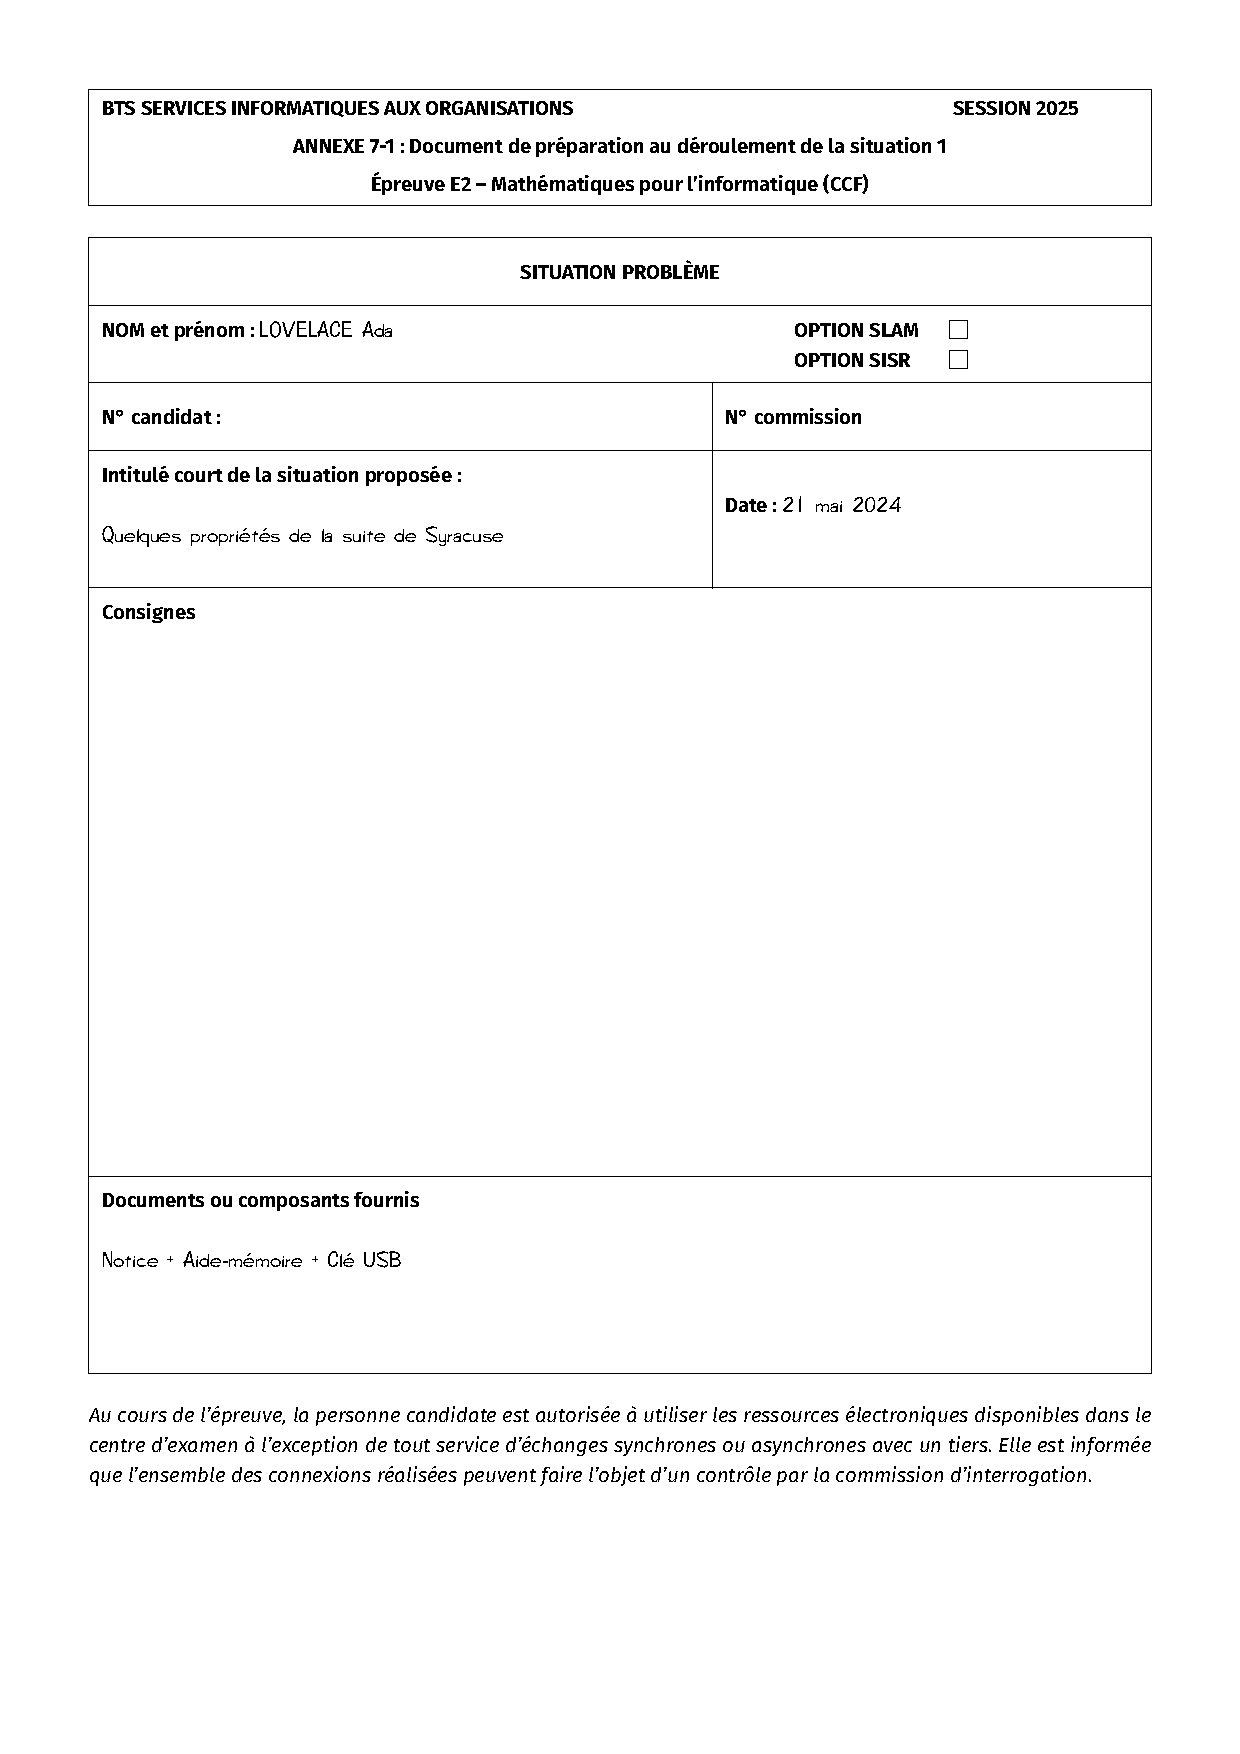
\includepdf[frame,pages=-,width=\textwidth]{ProfSio-doc-annexe71.pdf}

\newpage

\thispagestyle{empty}

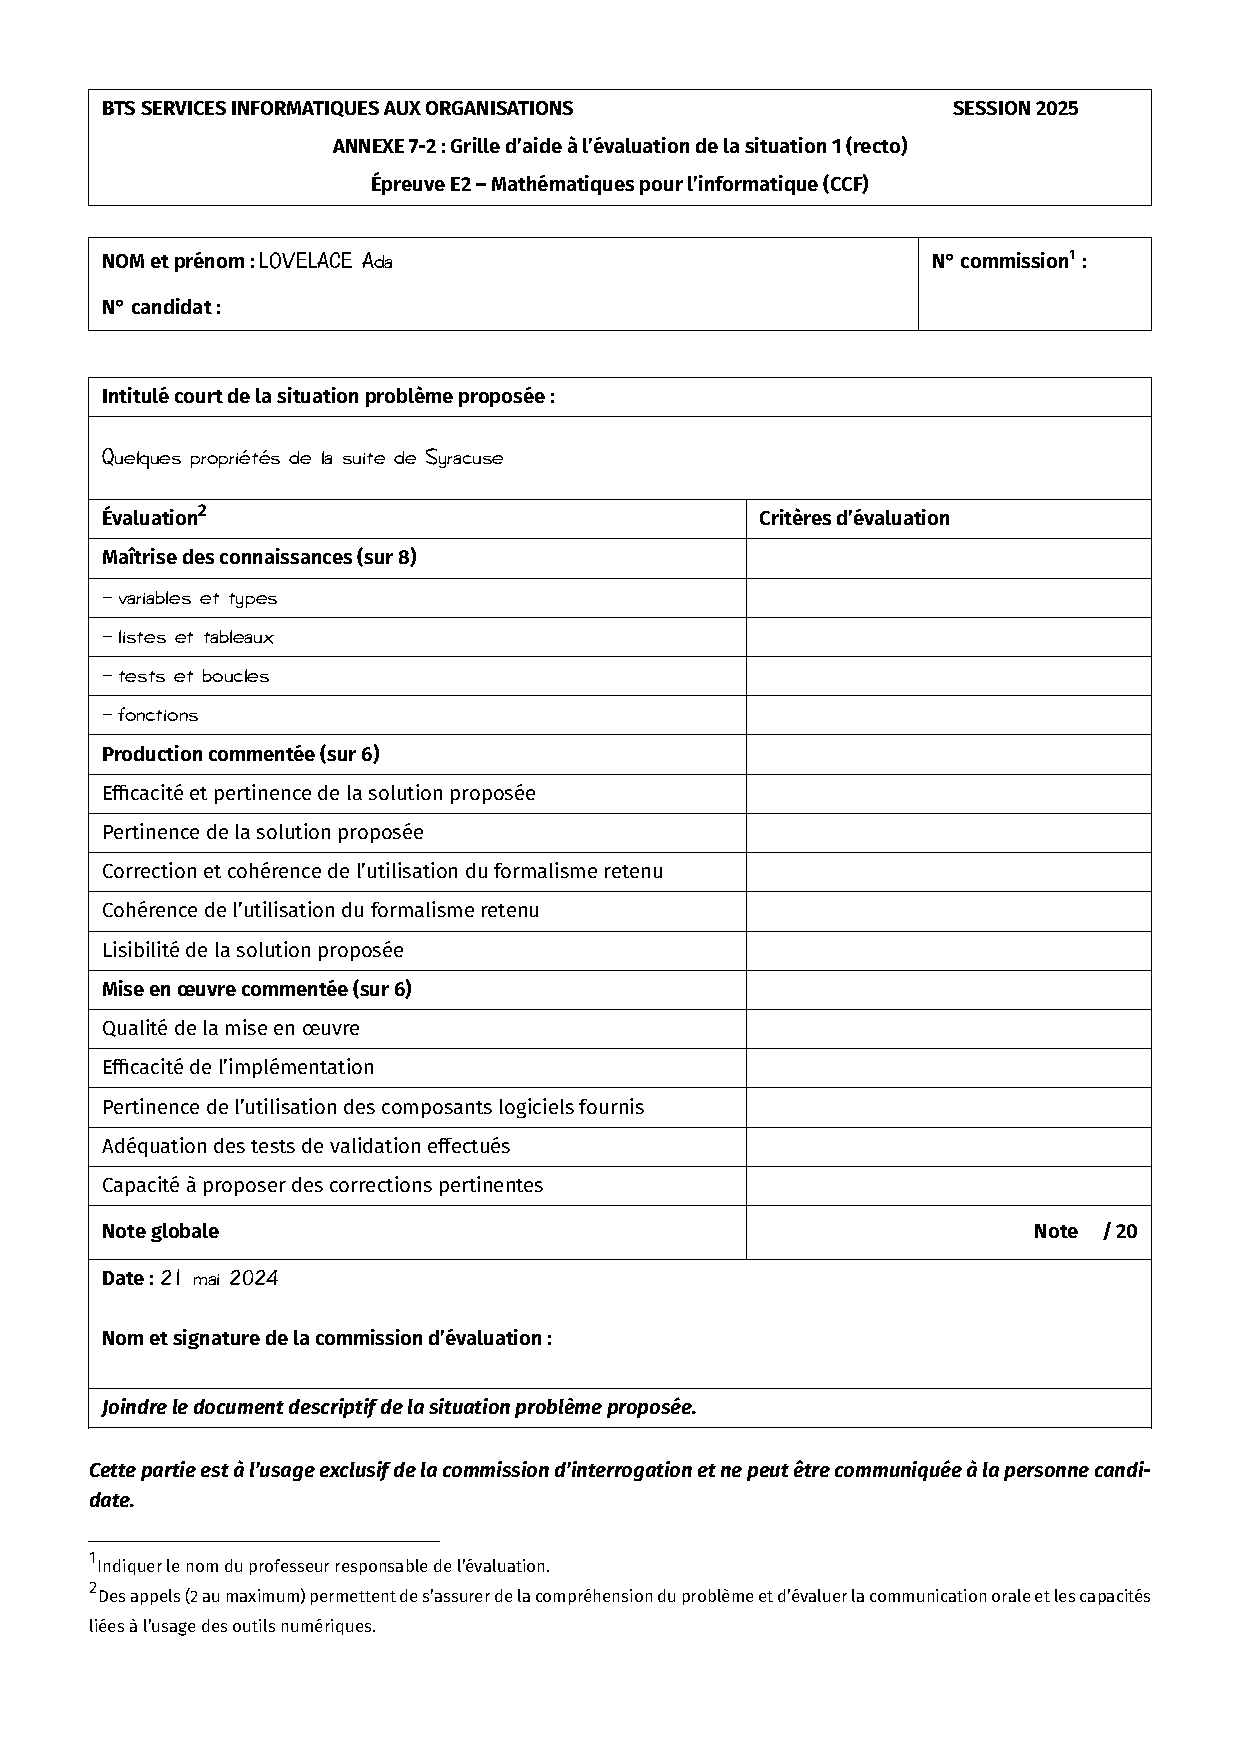
\includepdf[frame,pages=-,width=\textwidth]{ProfSio-doc-annexe72.pdf}

\newpage

\thispagestyle{empty}

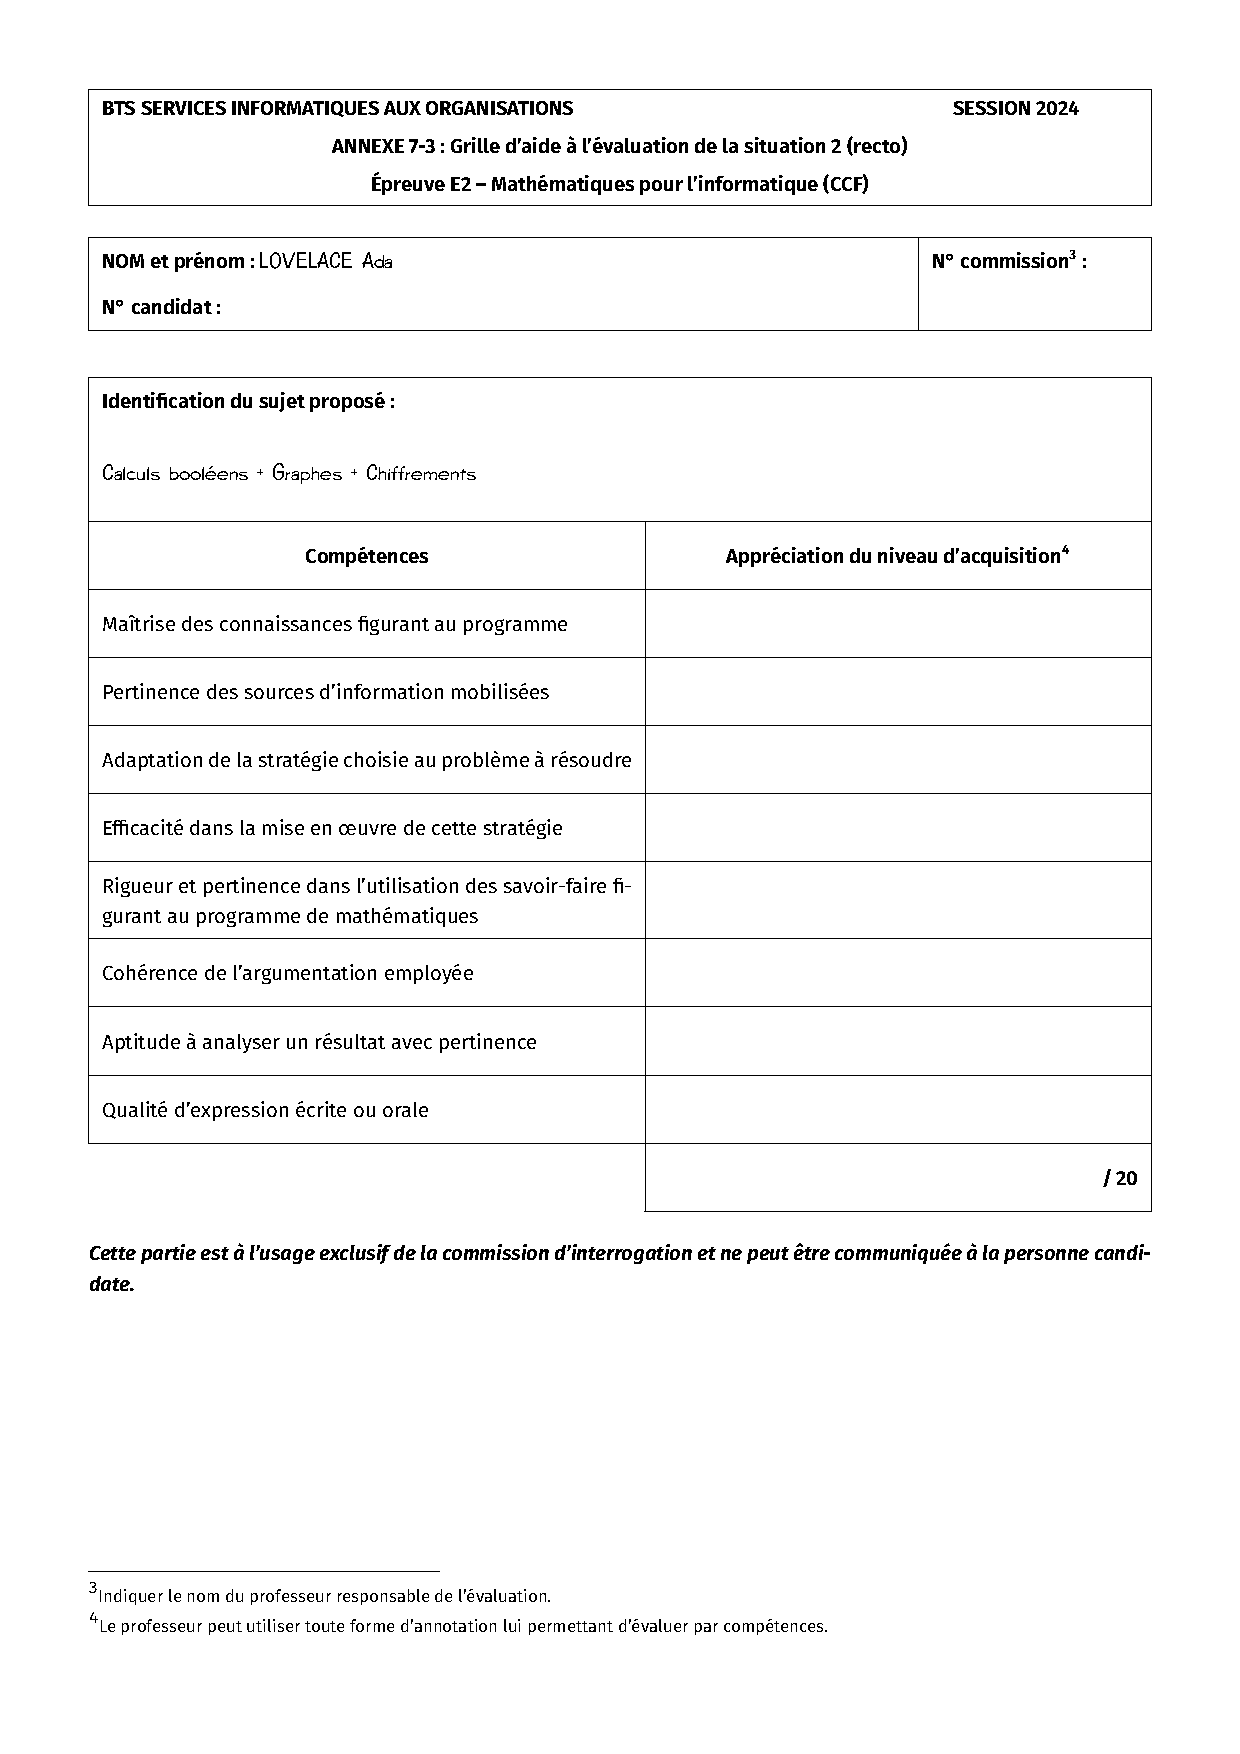
\includepdf[frame,pages=-,width=\textwidth]{ProfSio-doc-annexe73.pdf}

\end{document}